\documentclass[usenames, svgnames, dvipsnames]{scrartcl}
\usepackage{pgfplots}
\usepackage{emoji}
\usepackage[makeroom]{cancel}
\usepackage{simpler-wick}
\newcommand{\ech}{\mathbb{e}}
\newcommand{\gcod}{\mathfrak{D}}
\newcommand{\tz}{{t\tund{0}}}
\newcommand{\php}[1]{\phi_{#1}^+}
\newcommand{\phm}[1]{\phi_{#1}^-}
\newcommand{\fp}{\triangle}
\newcommand{\pho}{\phi_1}
\newcommand{\phii}{\phi_2}
\newcommand{\phiii}{\phi_3}
\newcommand{\phiv}{\phi_4}
\newcommand{\phv}{\phi_5}
\newcommand{\phvi}{\phi_6}
\newcommand{\ti}{{t\tund{1}}}
\newcommand{\tii}{{t\tund{2}}}
\newcommand{\tiii}{{t\tund{3}}}
\newcommand{\tiv}{{t\tund{4}}}
\newcommand{\tv}{{t\tund{5}}}
\usepackage{mathbbol}
\newcommand{\iqe}{iq\ech}
\newcommand{\vph}{\varphi}
\newcommand{\MH}{\mathrm{H}}
\newcommand{\ut}{\uptau}
\newcommand{\phint}{\phi\tund{I}}
\usepackage{simpler-wick}
\usepackage{mathrsfs}
\usepackage{mathtools}
\usepackage{booktabs} % For better table formatting
\usepackage{calc}
\usepackage{Style_File}

\newcommand{\crai}{\hat{c}\tund{A,i}^\dagger}
\newcommand{\annai}{\hat{c}\tund{A,i}}
\newcommand{\crbi}{\hat{c}\tund{B,i}^\dagger}
\newcommand{\annbi}{\hat{c}\tund{B,i}}

\newcommand{\crar}{\hat{c}\tund{A,r}^\dagger}
\newcommand{\annar}{\hat{c}\tund{A,r}}
\newcommand{\crbr}{\hat{c}\tund{B,r}^\dagger}
\newcommand{\annbr}{\hat{c}\tund{B,r}}


\newcommand{\crak}{\hat{c}\tund{A,k}^\dagger}
\newcommand{\annak}{\hat{c}\tund{A,k}}
\newcommand{\crbk}{\hat{c}\tund{B,k}^\dagger}
\newcommand{\annbk}{\hat{c}\tund{B,k}}


% \newcommand{\myeq}[1]{\stackrel{\mathclap{\tiny\mbox{#1}}}{=}}
\newcommand{\crakd}{\hat{c}\tund{A,k'}^\dagger}
\newcommand{\annakd}{\hat{c}\tund{A,k'}}
\newcommand{\crbkd}{\hat{c}\tund{B,k'}^\dagger}
\newcommand{\annbkd}{\hat{c}\tund{B,k'}}


\newcommand{\craip}{\hat{c}\tund{A,i+1}^\dagger}
\newcommand{\annaip}{\hat{c}\tund{A,i+1}}
\newcommand{\crbip}{\hat{c}\tund{B,i+1}^\dagger}
\newcommand{\annbip}{\hat{c}\tund{B,i+1}}
\newcommand{\craim}{\hat{c}\tund{A,i-1}^\dagger}
\newcommand{\annaim}{\hat{c}\tund{A,i-1}}
\newcommand{\crbim}{\hat{c}\tund{B,i-1}^\dagger}
\newcommand{\annbim}{\hat{c}\tund{B,i-1}}


\newcommand{\ad}[1]{a_{#1}^\dagger}
\usepackage{fancyhdr}
\usepackage{tikz-feynman}
\newcommand{\pdx}{\vb{p}\cdot \vb{x}}
\newcommand{\creap}{{\hat{a}_{\vb{p}}}^{s\dagger}}
\newcommand{\annap}{{\hat{a}_{\vb{p}}}^{s}}
\newcommand{\crebp}{{\hat{b}_{\vb{p}}}^{s\dagger}}
\newcommand{\annbp}{{\hat{b}_{\vb{p}}}^{s}}


\newcommand{\creapr}{{\hat{a}_{\vb{p}}}^{r\dagger}}
\newcommand{\annapr}{{\hat{a}_{\vb{p}}}^{r}}
\newcommand{\crebpr}{{\hat{b}_{\vb{p}}}^{r\dagger}}
\newcommand{\annbpr}{{\hat{b}_{\vb{p}}}^{r}}

\newcommand{\creampr}{{\hat{a}_{-\vb{p}}}^{r\dagger}}
\newcommand{\annampr}{{\hat{a}_{-\vb{p}}}^{r}}
\newcommand{\crebmpr}{{\hat{b}_{-\vb{p}}}^{r\dagger}}
\newcommand{\annbmpr}{{\hat{b}_{-\vb{p}}}^{r}}
\newcommand{\acomtr}[2]{\{#1,#2\}}
\newcommand{\pdy}{\vb{p}\cdot \vb{y}}
\newcommand{\qdy}{\vb{q}\cdot \vb{y}}

\newcommand{\qdx}{\vb{q}\cdot \vb{x}}
\newcommand{\creaq}{{\hat{a}_{\vb{q}}}^{s\dagger}}
\newcommand{\annaq}{{\hat{a}_{\vb{q}}}^{s}}
\newcommand{\crebq}{{\hat{b}_{\vb{q}}}^{s\dagger}}
\newcommand{\annbq}{{\hat{b}_{\vb{q}}}^{s}}
\usepackage{dashrule}
\newcommand{\creaqr}{{\hat{a}_{\vb{q}}}^{r\dagger}}
\newcommand{\annaqr}{{\hat{a}_{\vb{q}}}^{r}}
\newcommand{\crebqr}{{\hat{b}_{\vb{q}}}^{r\dagger}}
\newcommand{\annbqr}{{\hat{b}_{\vb{q}}}^{r}}

\newcommand{\creamqr}{{\hat{a}_{-\vb{q}}}^{r\dagger}}
\newcommand{\annamqr}{{\hat{a}_{-\vb{q}}}^{r}}
\newcommand{\crebmqr}{{\hat{b}_{-\vb{q}}}^{r\dagger}}
\newcommand{\annbmqr}{{\hat{b}_{-\vb{q}}}^{r}}

% \newcommand{\crebp}{def}
\newenvironment{bMatrix}[1]{%
\bmatrix\array{#1}\hspace*{-0.5\arraycolsep}}%
{\endarray\endbmatrix}
\newcommand{\tund}[1]{_{\text{\tiny #1}}}
\newcommand{\uep}{\upepsilon}
\newcommand{\sbo}[1]{\scalebox{0.56}{#1}}
\newcommand{\gsl}[1]{\cancel{#1}}
\usepackage{tensor}
\usepackage{array}
\usepackage{lmodern}
\definecolor{violet}{rgb}{0.5,0.27,0.45}
\newcommand{\hint}{\MH\tund{I}}
\newcommand{\fvec}[1]{\vb{#1}}
\newcommand{\cre}[1]{\hat{a}_{#1}^\dagger}
\newcommand{\ann}[1]{\hat{a}_{#1}}

\newcommand{\crep}{\hat{a}_{\vb{p}}^\dagger}
\newcommand{\annp}{\hat{a}_{\vb{p}}}
\newcommand{\fo}{\hat{\phi}}
\newcommand{\crepd}{\hat{a}_{\vb{p}'}^\dagger}
\newcommand{\annpd}{\hat{a}_{\vb{p}'}}
\newcommand{\vac}{\ket{\Omega}}
\newcommand{\vacb}{\bra{\Omega}}
\newcommand{\cremp}{\hat{a}_{\vb{-p}}^\dagger}
\newcommand{\annmp}{\hat{a}_{\vb{-p}}}

\newcommand{\crempd}{\hat{a}_{\vb{-p}'}^\dagger}
\newcommand{\annmpd}{\hat{a}_{\vb{-p}'}}

\newcommand{\tvec}[1]{\vb{{#1}}}
\renewcommand{\aa}[1]{a_{#1}}
\newcommand{\overbar}[1]{\mkern 1.5mu\overline{\mkern-1.5mu{#1}\mkern-1.5mu}\mkern 1.5mu}
\newcommand{\dadj}[1]{\overbar{#1}}
\newcommand{\bili}[1]{\dadj{\Psi}\ #1 \ \Psi}
\newcommand{\bilin}[3]{\dadj{\Psi}_{#1}\ #3 \ \Psi_{#2}}
\newcommand{\lrep}{\mathrm{S}[\Lambda]}
\newcommand{\lrepd}{\mathrm{S}^\dagger[\Lambda]}
\newcommand{\lrepinv}{\mathrm{S}^{-1}[\Lambda]}
\newcolumntype{P}[1]{>{\centering\arraybackslash}p{#1}}
% Recommended preamble:
\usetikzlibrary{arrows.meta}
\usetikzlibrary{backgrounds}
\usepgfplotslibrary{patchplots}
\usepgfplotslibrary{fillbetween}
\pgfplotsset{%
    layers/standard/.define layer set={%
        background,axis background,axis grid,axis ticks,axis lines,axis tick labels,pre main,main,axis descriptions,axis foreground%
    }{
        grid style={/pgfplots/on layer=axis grid},%
        tick style={/pgfplots/on layer=axis ticks},%
        axis line style={/pgfplots/on layer=axis lines},%
        label style={/pgfplots/on layer=axis descriptions},%
        legend style={/pgfplots/on layer=axis descriptions},%
        title style={/pgfplots/on layer=axis descriptions},%
        colorbar style={/pgfplots/on layer=axis descriptions},%
        ticklabel style={/pgfplots/on layer=axis tick labels},%
        axis background@ style={/pgfplots/on layer=axis background},%
        3d box foreground style={/pgfplots/on layer=axis foreground},%
    },
}
\newcommand{\amstitle}[1]{%
  {\Large\MakeUppercase{#1}}% First letter large, rest small caps (simplified)
  % OR for true small caps:
  % {\Large\MakeUppercase{\expandafter\@firstofone#1}\scshape\MakeLowercase{#1}}%
}
\usepackage[left = 0.8in,
right = 0.6in,
bottom = 0.8in,
top = 0.8in,
a4paper]{geometry}


\fancyhead[L,C]{}
\fancyhead[R]{PH4101}
\usepackage[hidelinks]{hyperref}
\hypersetup{colorlinks=true,linkcolor=cyan!80!black, citecolor=YellowOrange,urlcolor=cyan!80!black}
\fancyhead[L]{Assignment 03}
\fancyhead[C]{ Condensed Matter}
\fancyfoot[C]{\thepage}
\fancyfoot[R,L]{}
\usetikzlibrary{calc}
\pagestyle{fancy}
\newcommand{\delt}[2]{\tensor{\delta}{^{#1}_{#2}}}
\newcommand{\vact}{\ket{\widetilde{\Omega}}}
\newcommand{\vactb}{\bra{\widetilde{\Omega}}}
\newcommand{\meas}[1]{\frac{\dd^3\tvec{#1}}{(2\pi)^3}}
\newcommand{\tvp}{\tvec{p}}
\newcommand{\tvpd}{\tvec{p}'}
\newcommand{\ddelt}[1]{\delta^{(3)}(#1)}
\newcommand{\myeq}[1]{\mathrel{\stackrel{\makebox[0pt]{\mbox{\normalfont\tiny #1}}}{=}}}\newcommand{\omp}{\omega_{\tvp}}
\newcommand{\ompd}{\omega_{\tvpd}}
\renewcommand{\headrulewidth}{0.4pt}
\definecolor{titleblue}{RGB}{0, 80, 120}
\usepackage{longtable} 

\renewcommand{\fdv}[2]{\frac{\delta #1}{\delta #2}}
\begin{document}
\begin{center}
    {\Large \textbf{\sffamily Assignment 03: Condensed Matter Physics }} \\[0.2cm]
   {\sffamily Sagnik Seth \hspace{0.4cm} 22MS026}\\[1cm]
\end{center}
% \begin{definition}[Kronig-Penney Model]


% Consider a one-dimensional periodic potential consisting of a sequence of rectangular barriers of height \(U\), width \(b\), and period \(a\):

% \[
% V(x)=\begin{cases}U,&0\leq x<b\pmod{a},\\ 0,&b\leq x<a\pmod{a}.\end{cases}
% \]

% \begin{enumerate}
%    { \item[(a)] Choosing values for \(U\), \(b\), \(a\) so that (\(0<b<a\)), numerically solve the Kronig-Penney dispersion to obtain \(E(\mathbf{k})\) within the first Brillouin zone. Plot the dispersion and clearly indicate the allowed bands and band gaps. Mark the lowest two energy bands and the zone boundaries at \(k=\pm\pi/a\).

%     \item[(b)] Consider the limiting case of the Kronig-Penney model where \(b\to 0\) and \(U\rightarrow\infty\), while keeping the product \(V_{0}\equiv Ub\) constant. In this limit, the potential reduces to a Dirac comb, and the dispersion relation takes the form 
%     \[
%     \cos(ka)=\cos(qa)+\frac{maV_{0}}{\hbar^{2}}\frac{\sin(qa)}{qa},
%     \]
%     where \(q\) is the wave vector inside the potential wells. Now, by allowing the wave vector \(k\) to take complex values, numerically demonstrate that the corresponding energy solutions lie within the forbidden energy gaps of the band structure. (It is sufficient to perform the numerical analysis within the first energy band gap.)}
% \end{enumerate}
% \end{definition}
\noindent
\underline{\textbf{{\sffamily Solution 1: Kronig-Penney Model}}}
\begin{figure}[H]
    \centering 
    

% Pattern Info
 
\tikzset{
pattern size/.store in=\mcSize, 
pattern size = 5pt,
pattern thickness/.store in=\mcThickness, 
pattern thickness = 0.3pt,
pattern radius/.store in=\mcRadius, 
pattern radius = 1pt}
\makeatletter
\pgfutil@ifundefined{pgf@pattern@name@_a06p5nyc3}{
\pgfdeclarepatternformonly[\mcThickness,\mcSize]{_a06p5nyc3}
{\pgfqpoint{0pt}{0pt}}
{\pgfpoint{\mcSize+\mcThickness}{\mcSize+\mcThickness}}
{\pgfpoint{\mcSize}{\mcSize}}
{
\pgfsetcolor{\tikz@pattern@color}
\pgfsetlinewidth{\mcThickness}
\pgfpathmoveto{\pgfqpoint{0pt}{0pt}}
\pgfpathlineto{\pgfpoint{\mcSize+\mcThickness}{\mcSize+\mcThickness}}
\pgfusepath{stroke}
}}
\makeatother

% Pattern Info
 
\tikzset{
pattern size/.store in=\mcSize, 
pattern size = 5pt,
pattern thickness/.store in=\mcThickness, 
pattern thickness = 0.3pt,
pattern radius/.store in=\mcRadius, 
pattern radius = 1pt}
\makeatletter
\pgfutil@ifundefined{pgf@pattern@name@_g7gb3168j}{
\pgfdeclarepatternformonly[\mcThickness,\mcSize]{_g7gb3168j}
{\pgfqpoint{0pt}{0pt}}
{\pgfpoint{\mcSize+\mcThickness}{\mcSize+\mcThickness}}
{\pgfpoint{\mcSize}{\mcSize}}
{
\pgfsetcolor{\tikz@pattern@color}
\pgfsetlinewidth{\mcThickness}
\pgfpathmoveto{\pgfqpoint{0pt}{0pt}}
\pgfpathlineto{\pgfpoint{\mcSize+\mcThickness}{\mcSize+\mcThickness}}
\pgfusepath{stroke}
}}
\makeatother

% Pattern Info
 
\tikzset{
pattern size/.store in=\mcSize, 
pattern size = 5pt,
pattern thickness/.store in=\mcThickness, 
pattern thickness = 0.3pt,
pattern radius/.store in=\mcRadius, 
pattern radius = 1pt}
\makeatletter
\pgfutil@ifundefined{pgf@pattern@name@_ut6g9j4ba}{
\pgfdeclarepatternformonly[\mcThickness,\mcSize]{_ut6g9j4ba}
{\pgfqpoint{0pt}{0pt}}
{\pgfpoint{\mcSize+\mcThickness}{\mcSize+\mcThickness}}
{\pgfpoint{\mcSize}{\mcSize}}
{
\pgfsetcolor{\tikz@pattern@color}
\pgfsetlinewidth{\mcThickness}
\pgfpathmoveto{\pgfqpoint{0pt}{0pt}}
\pgfpathlineto{\pgfpoint{\mcSize+\mcThickness}{\mcSize+\mcThickness}}
\pgfusepath{stroke}
}}
\makeatother

% Pattern Info
 
\tikzset{
pattern size/.store in=\mcSize, 
pattern size = 5pt,
pattern thickness/.store in=\mcThickness, 
pattern thickness = 0.3pt,
pattern radius/.store in=\mcRadius, 
pattern radius = 1pt}
\makeatletter
\pgfutil@ifundefined{pgf@pattern@name@_g24ecjuur}{
\pgfdeclarepatternformonly[\mcThickness,\mcSize]{_g24ecjuur}
{\pgfqpoint{0pt}{0pt}}
{\pgfpoint{\mcSize+\mcThickness}{\mcSize+\mcThickness}}
{\pgfpoint{\mcSize}{\mcSize}}
{
\pgfsetcolor{\tikz@pattern@color}
\pgfsetlinewidth{\mcThickness}
\pgfpathmoveto{\pgfqpoint{0pt}{0pt}}
\pgfpathlineto{\pgfpoint{\mcSize+\mcThickness}{\mcSize+\mcThickness}}
\pgfusepath{stroke}
}}
\makeatother
\tikzset{every picture/.style={line width=0.75pt}} %set default line width to 0.75pt        

\begin{tikzpicture}[x=0.75pt,y=0.75pt,yscale=-1,xscale=1]
%uncomment if require: \path (0,300); %set diagram left start at 0, and has height of 300

%Shape: Rectangle [id:dp801825587475429] 
\draw  [color={rgb, 255:red, 255; green, 255; blue, 255 }  ,draw opacity=1 ][pattern=_a06p5nyc3,pattern size=15pt,pattern thickness=0.75pt,pattern radius=0pt, pattern color={rgb, 255:red, 0; green, 0; blue, 0}] (455.01,58) -- (525.01,58) -- (525.01,138.45) -- (455.01,138.45) -- cycle ;
%Shape: Rectangle [id:dp2785151477132142] 
\draw  [color={rgb, 255:red, 255; green, 255; blue, 255 }  ,draw opacity=1 ][pattern=_g7gb3168j,pattern size=15pt,pattern thickness=0.75pt,pattern radius=0pt, pattern color={rgb, 255:red, 0; green, 0; blue, 0}] (339.19,58) -- (409.19,58) -- (409.19,138.45) -- (339.19,138.45) -- cycle ;
%Shape: Rectangle [id:dp6375387079850631] 
\draw  [color={rgb, 255:red, 255; green, 255; blue, 255 }  ,draw opacity=1 ][pattern=_ut6g9j4ba,pattern size=15pt,pattern thickness=0.75pt,pattern radius=0pt, pattern color={rgb, 255:red, 0; green, 0; blue, 0}] (223.62,58) -- (293.62,58) -- (293.62,138.45) -- (223.62,138.45) -- cycle ;
%Shape: Rectangle [id:dp10300641106250974] 
\draw  [color={rgb, 255:red, 255; green, 255; blue, 255 }  ,draw opacity=1 ][pattern=_g24ecjuur,pattern size=15pt,pattern thickness=0.75pt,pattern radius=0pt, pattern color={rgb, 255:red, 0; green, 0; blue, 0}] (109.92,58) -- (179.92,58) -- (179.92,138.45) -- (109.92,138.45) -- cycle ;
%Shape: Pulse Wave Form [id:dp4138641938139961] 
\draw  [color={rgb, 255:red, 255; green, 0; blue, 31 }  ,draw opacity=1 ][line width=1.5]  (66.29,138.45) -- (109.99,138.45) -- (109.99,58) -- (179.92,58) -- (179.92,138.45) -- (223.62,138.45) ;
%Shape: Pulse Wave Form [id:dp8918434817529324] 
\draw  [color={rgb, 255:red, 255; green, 0; blue, 31 }  ,draw opacity=1 ][line width=1.5]  (182.03,138.45) -- (225.74,138.45) -- (225.74,58) -- (295.67,58) -- (295.67,138.45) -- (339.37,138.45) ;
%Shape: Pulse Wave Form [id:dp9593409165583205] 
\draw  [color={rgb, 255:red, 255; green, 0; blue, 31 }  ,draw opacity=1 ][line width=1.5]  (295.56,138.45) -- (339.26,138.45) -- (339.26,58) -- (409.19,58) -- (409.19,138.45) -- (452.89,138.45) ;
%Shape: Pulse Wave Form [id:dp6916678635719636] 
\draw  [color={rgb, 255:red, 255; green, 0; blue, 31 }  ,draw opacity=1 ][line width=1.5]  (411.3,138.45) -- (455.01,138.45) -- (455.01,58) -- (524.93,58) -- (524.93,138.45) -- (568.64,138.45) ;


% Text Node
\draw (577.09,136.4) node [anchor=north west][inner sep=0.75pt]    {$\dotsc $};
% Text Node
\draw (37.88,136.4) node [anchor=north west][inner sep=0.75pt]    {$\dotsc $};
% Text Node
\draw (220.34,144.85) node [anchor=north west][inner sep=0.75pt]    {$0$};
% Text Node
\draw (293,144.85) node [anchor=north west][inner sep=0.75pt]    {$b$};
% Text Node
\draw (334,144.85) node [anchor=north west][inner sep=0.75pt]    {$a$};
% Text Node
\draw (210,47.4) node [anchor=north west][inner sep=0.75pt]    {$U$};


\end{tikzpicture}

\end{figure}
\noindent
(a) The dispersion relation obtained from the class for the Kronig-Penney model was 
\begin{equation*}
    \cos(ka) = \cos(\alpha d)\cosh(\beta b) + \frac{\beta^2-\alpha^2}{2\alpha\beta}\sin(\alpha d)\sinh(\beta b)
\end{equation*}
where $d=a-b$ and for simplicity we take $m=\hbar=1$. We have the following 
 $$\vartriangleright\ \alpha =\sqrt{\frac{2mE}{\hbar^2}} =\sqrt{2E}\qquad\vartriangleright \beta =\sqrt{\frac{2m(U-E)}{\hbar^2}} =  \sqrt{2(U-E)}$$
We numerically found the roots of the above dispersion relation, taking the parameters
$$\vartriangleright\ a = 1.0\quad \vartriangleright\ b=0.04 \quad \vartriangleright\ U=80.0$$
\begin{figure}[H]
    \centering
    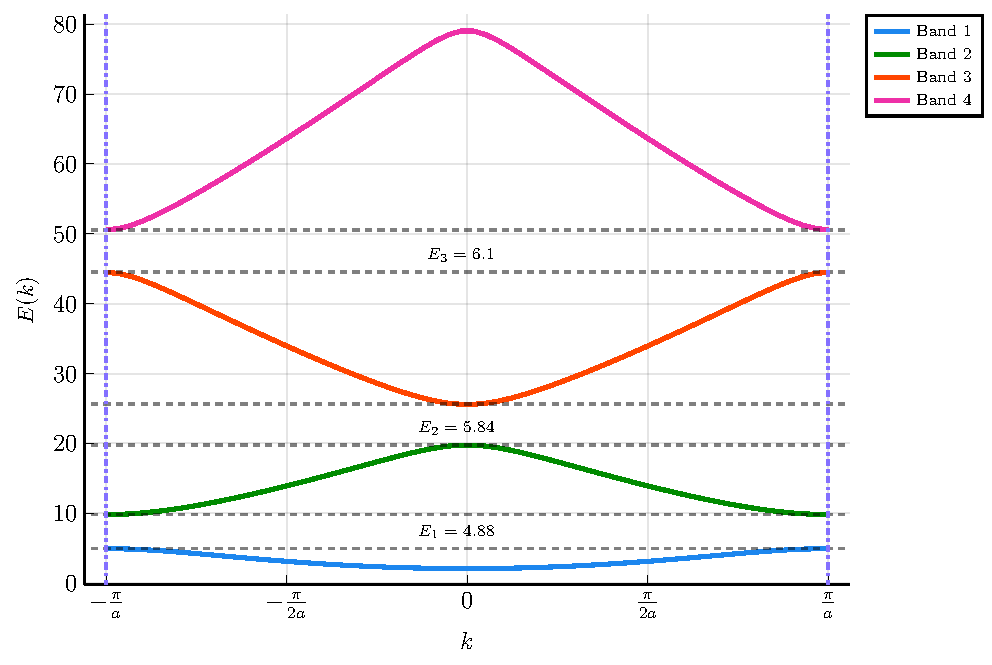
\includegraphics[scale=0.7]{Q1(a)plot.pdf}
    \caption{\textbf{Energy dispersion for Kronig-Penney model.} The figure shows the four lowest bands marked with different colors. The increasing bandgaps obtained for the above parameters are $\triangle E =4.88,5.84,6.1$ denoted in the plot. The dashed horizontal lines denote the energy band boundaries and the vertical lines denote the BZ boundaries at $\pm \sfrac{\pi}{a}$}
\end{figure}
\noindent 
(b) Consider the dispersion relation for the KP model again 
\begin{equation*}
    \cos(ka) = \cos(\alpha d)\cosh(\beta b) + \frac{\beta^2-\alpha^2}{2\alpha\beta}\sin(\alpha d)\sinh(\beta b)
\end{equation*}
Taking $m=\hbar^2=1$, in the limit $U\to \infty $ and $b\to 0$ keeping $Ub= V\tund{0}$ constant, we have 
$$\beta = \sqrt{2(U-E)} = \sqrt{2U}\qty(1 - \frac{E}{2U})\ \longrightarrow\ \beta b = \sqrt{2U}b - \frac{\sqrt{2}E}{\sqrt{U}} = \frac{\sqrt{2}(V\tund{0}-E)}{\sqrt{U}} \xrightarrow{U\to \infty} 0$$
Hence the arguments of the hyperbolic trig functions can be taken to be `small' and expanded upto linear order in $\beta b$ from where we get: $\sinh(\beta b) \approx \beta b \qquad  \cosh(\beta b) \approx 1 $\\[0.2cm]
Also note that $\sin(\alpha(a-b)) \approx \sin(\alpha a)$ and $\cos(\alpha(a-b))\approx \cos(\alpha a)$ since $b\to 0$. Due to the same reason, we have 
$$\frac{b}{2}(\beta^2-\alpha^2) = \frac{b}{2}\qty(2(U-E)-2E) = b\qty[U - 2E] = Ub - 2Eb = V\tund{0} - 2Eb \xrightarrow{b\to 0} V\tund{0} $$
Substituting everything in the dispersion relation above we obtain:
\begin{align*}
        \cos(ka) &= \cos(\alpha d)\cosh(\beta b) + \frac{\beta^2-\alpha^2}{2\alpha\beta}\sin(\alpha d)\sinh(\beta b)=\cos(\alpha a)\times 1 + \frac{\cancel{2}V\tund{0}}{\cancel{2}\cancel{b}\alpha\cancel{\beta}}\sin(\alpha a)\times(\cancel{\beta}\cancel{b})
\end{align*}
Reintroducing terms for $m$ and $\hbar$ we obtain 
$$\boxed{\cos(ka) = \cos(\alpha a) + \frac{maV\tund{0} }{\hbar^2}\frac{\sin(\alpha a)}{\alpha a}}$$
We now take $k$ to be complex and try to find the allowable energy solutions. 
\begin{figure}[H]
    \centering
    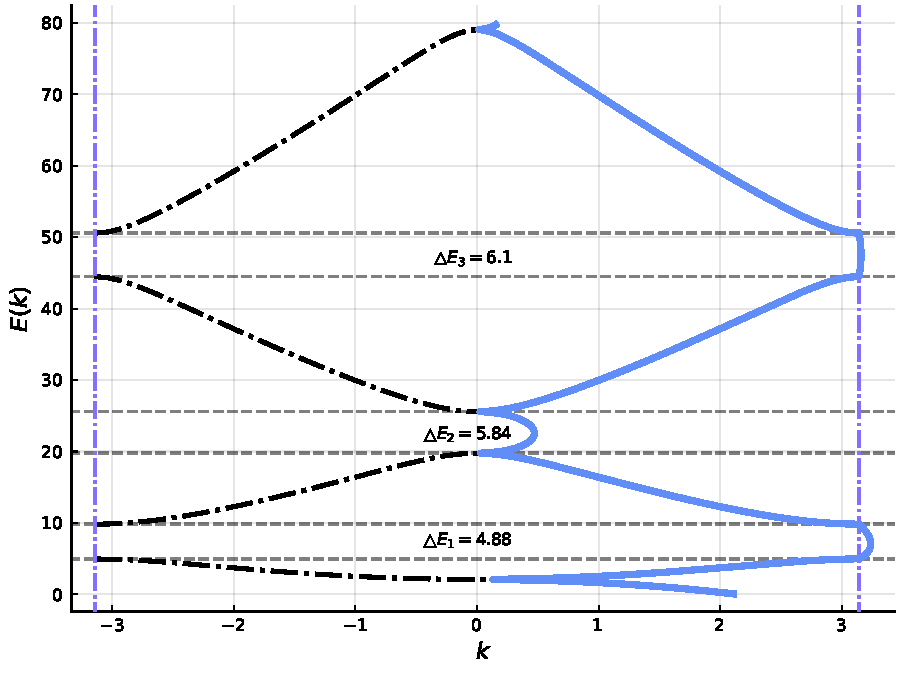
\includegraphics[scale=0.65]{Q1(b).pdf}
    \caption{\textbf{Dispersion for complex $\mathbf{k}$.} The dashed black lines corresponds to the bands previously obtain with real wave-vectors. The blue plot denote the energy solution vs. $|k|$ where $k \in \mathbb{C}$. We can see that for some $k\in \mathbb{C}$ we have $E$ inside the forbidden region (bandgap). }
\end{figure}
\vspace{0.2cm}
% \begin{definition}[2D Square Lattice]
%     Consider a two-dimensional square lattice with lattice constant \(a\), where each site hosts a single orbital \(|m,n\rangle\), with \(m\) and \(n\) denoting the lattice indices along the \(x\) and \(y\)-directions, respectively. Electrons can hop between nearest neighbours with hopping amplitude \(t\), and each site has an on-site energy \(\varepsilon\tund{0}\). The tight-binding Hamiltonian is given by:
% \[
% H=-t\sum_{m,n}\left(|m+1,n\rangle\left\langle m,n\right|+|m,n+1 \rangle\left\langle m,n\right|+\text{h.c.}\right)+\varepsilon\tund{0}\sum_{m,n}|m,n \rangle\left\langle m,n\right|.
% \]

% \begin{enumerate}
%     \item[(a)] Derive the dispersion relation \(E(\mathbf{k})\) using Bloch's theorem, and plot the equal-energy contours in the \(k_{x}-k_{y}\) plane within the first Brillouin zone, i.e., for \(-\pi/a<k_{x}<\pi/a\) and \(-\pi/a<k_{y}<\pi/a\).
    
%     \item[(b)] Compute the density of states (DOS) corresponding to the energy band. Examine if there are any singularities that appear, and if so, comment on the nature of these van Hove singularities.
    
%     \item[(c)] Consider each site is populated on average by a single electron (half-filled case) and determine the Fermi energy \(E_{F}\) and the corresponding Fermi momentum \(\mathbf{k}_{F}\). Plot the Fermi surface in the first Brillouin zone.
% \end{enumerate}

% \end{definition}
% \noindent
% \textit{Answer.}\\[0.2cm]
\noindent
\underline{\textbf{{\sffamily Solution 2: 2D Square Lattice}}}
\\[0.3cm]
\noindent
(a) Let us consider the state with momentum ket $\ket{\vb{k}} \equiv \ket{k\tund{x}, k\tund{y}}$ and from Bloch's theorem, we can expand it as 
\begin{align*}
    \ket{\vb{k}} = \frac{1}{\sqrt{N}} \sum\limits_{\vb{R}} e^{i \vb{k}\cdot \vb{R}} \ket{\vb{R}}\quad \longleftrightarrow\quad \ket{k\tund{x}, k\tund{y}} = \frac{1}{\sqrt{N}} \sum\limits_{m,n} e^{ia (k\tund{x} m +k\tund{y}n )} \ket{m,n}
\end{align*}
Now, substituting this in the Hamiltonian gives us 
\begin{align*}
        H\ket{\vb{k}} &= -\frac{t}{\sqrt{N}} \sum\limits_{m,n,p,q}e^{ia(k\tund{x}p + k\tund{y}q )} \Big\{\ket{m+1,n}\braket{m,n|p,q}+\ket{m,n+1}\braket{m,n|p,q}+\\ &\qquad\qquad\qquad\qquad\quad\qquad\qquad\ket{m,n}\braket{m+1,n|p,q}+\ket{m,n}\braket{m,n+1|p,q}\Big\}\\ &\qquad\qquad\qquad\qquad\quad\hspace{4cm}+\varepsilon\tund{0}\sum\limits_{m,n,p,q} e^{ia(k\tund{x}p + k\tund{y}q )}\ket{m,n}\braket{m,n|p,q}
\end{align*}
Since the orbitals are localised we have the following condition: $\braket{m,n|p,q} = \delta_{mp}\delta_{nq}\quad \forall \ m,n,p,q$. Using this in the equation above we obtain: 
\begin{align*}
       H\ket{\vb{k}} &= -\frac{t}{\sqrt{N}} \sum\limits_{p,q}e^{ia(k\tund{x}p + k\tund{y}q )} \Big\{\ket{p+1,q}+\ket{p,q+1}+\ket{p-1,q}+\\ &\qquad\qquad\qquad\qquad\quad\qquad\qquad \ket{p,q-1}\Big\} +\varepsilon\tund{0} \sum\limits_{p,q}e^{ia(k\tund{x}p + k\tund{y}q )} \ket{p,q}\\
       &=-\frac{t}{\sqrt{N}} \sum\limits_{p,q}\qty(e^{ia(k\tund{x}(p-1) + k\tund{y}q )}+e^{ia(k\tund{x}p + k\tund{y}(q-1) )}+e^{ia(k\tund{x}(p+1) + k\tund{y}q )}+e^{ia(k\tund{x}p + k\tund{y}(q+1) )})\ket{p,q} + \varepsilon\tund{0}\ket{\vb{k}}\\
       &= -t\qty(e^{-iak\tund{x}} + e^{-iak\tund{y}}+e^{iak\tund{x}}+e^{iak\tund{y}})\sum\limits_{p,q}(e^{ia(k\tund{x}p + k\tund{y}q)})\ket{p,q}+ \varepsilon\tund{0}\ket{\vb{k}}=\qty[\varepsilon\tund{0}-2t\cos(k\tund{x}a) -2t \cos(k\tund{y}a)]\ket{\vb{k}}
\end{align*}
We obtain an eigen-equation for $\ket{\vb{k}}$ and the dispersion relation thus obtained is 
\begin{align*}
  \boxed{  E(\vb{k}) = \qty[\varepsilon\tund{0} -2t\cos(k\tund{x}a) -2t \cos(k\tund{y}a)]}
\end{align*}
\begin{figure}[H]
    \centering 
    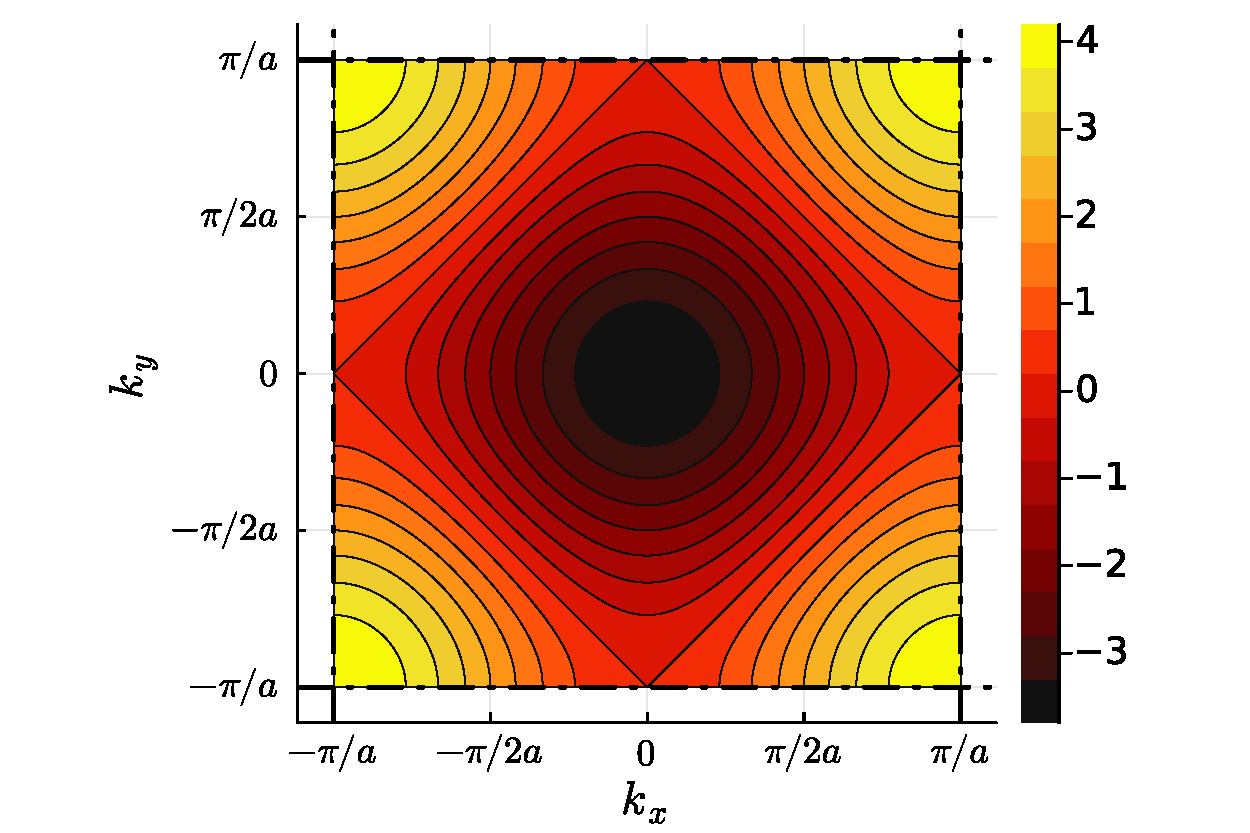
\includegraphics[scale=0.6]{Q2(a).pdf}
    \caption{\textbf{Dispersion for 2D Square lattice.} Energy contours for 2D suare lattice within the first BZ; parameters used $t=1.0, a=1.0,\varepsilon\tund{0}=0.2$. The dashed lines denote the BZ boundary at $\pm \frac{\pi}{a}$ }
\end{figure}
\noindent
(b) The density of states is given by the expression 
$$\rho(E) = \int\limits_{\vb{k} \in \text{BZ}} \frac{\dd^2 k}{(2\pi)^2}\ \delta(E- E(\vb{k}))$$
Using the dispersion relation found out before, we have for the DOS 
\begin{align*}
        \rho(E) =\frac{1}{(2\pi)^2} \int\limits_{-\sfrac{\pi}{a}}^{\sfrac{\pi}{a}} \dd k\tund{x} \int\limits_{-\sfrac{\pi}{a}}^{\sfrac{\pi}{a}} \dd k\tund{y} \ \delta(E-  \qty[\varepsilon\tund{0} -2t\cos(k\tund{x}a) -2t \cos(k\tund{y}a)])
\end{align*}
\begin{figure}[H]
    \centering
    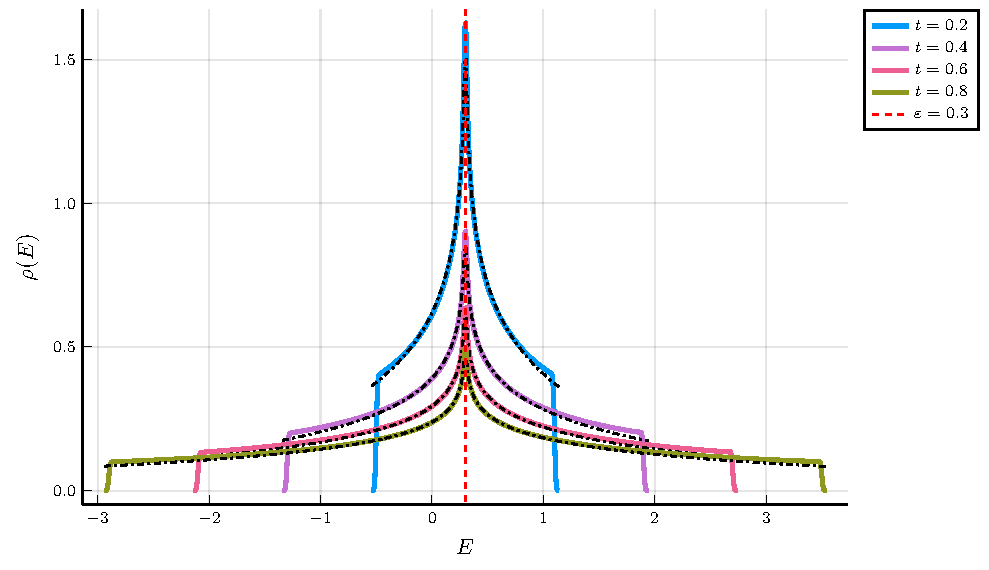
\includegraphics[scale=0.6]{Q2(van).pdf}
    \caption{\textbf{Density of states of 2D square lattice}. The plots are shown for various values of the hopping amplitude and $\varepsilon\tund{0}=0.3$. We can clearly see a singularity of the DOS at $E=\varepsilon\tund{0}$. The black lines are fit for the DOS with the logarithmic divergence $A-B\ln|E-\varepsilon\tund{0}$ }
\end{figure}
\noindent
In 2D, the density of states can alternately be defined as,
$$g(\varepsilon) = \frac{1}{(2\pi)^2}\int\limits_{\vb{k'}\in S(\varepsilon)} \frac{\dd^2 \vb{k}'}{|\vb{\nabla} E(\vb{k'})|}$$
where $S(\varepsilon)$ is the constant energy surface, that is, $S(\varepsilon) = \{\vb{k}| E(\vb{k}) = \varepsilon\}$. From the expression above, we can see that the integrand shows a potential singularity at points where there is an extrememum of energy, that is, $\nabla E = 0$.\\[0.2cm]
For our dispersion $E(k) = \varepsilon\tund{0}-2t(\cos(k\tund{x}a)+\cos(k\tund{y}a))$ we can see that:
$$\pdv{E}{k\tund{x}} = 2at\sin(k\tund{x}a) = 0\implies k\tund{x} = 0,\pm \frac{\pi}{a} $$
Similar result holds for $\pdv{E}{k\tund{y}}$ too. However we leave the point $-\frac{\pi}{a}$ since this is equivalent to $\frac{\pi}{a}$ due to the periodicity of the BZ. \\[0.2cm]
Now, we have potentially the points $\vb{k} = (0,0), (0,\pi/a), (\pi/a,0), (\pi/a,\pi/a)$. Out of these, $(0,0)$ and $(\pi/a,\pi/a)$ are the minima and maxima since $E = \varepsilon\tund{0}-2t$ and $E = \varepsilon\tund{0}+2t$ respectively at these points, and singularities do not occur at these points. The other two points are the \textit{saddle points} where the singularities occur and the DOS shows a logarithmic divergence around the singularity point, $E = \varepsilon\tund{0} - 2t(-1 +1) = \varepsilon\tund{0}$:
$$g(E)\sim -\ln|E-\varepsilon\tund{0}| \quad \text{where } E\text{ is close to $\varepsilon\tund{0}$}$$
(c) We consider the half-filling of electrons (with spin $\frac{1}{2}$) in this case. Thus for $N$ sites we will have $N$ momentum states with momentum $\vb{k}$ and we will have total $2N$ electrons occupying these states. Consider a transformation $\vb{k}\to \vb{k} + \qty(\frac{\pi}{a}, \frac{\pi}{a})$. The energy for this state is, 
$$E(\vb{k}') = \varepsilon\tund{0} -2t \qty[\cos(\qty(k\tund{x}+\frac{\pi}{a})a)+\cos(\qty(k\tund{x}+\frac{\pi}{a})a)]= \varepsilon\tund{0} +2t \qty[\cos(k\tund{x}a)+\cos(k\tund{x}a)] = 2\varepsilon\tund{0}-E(\vb{k})$$
We obtained a relation that for any such transformation $\vb{k}\to \vb{k} + \qty(\frac{\pi}{a}, \frac{\pi}{a})$, we have $E(\vb{k}') + E(\vb{k}) = 2\varepsilon\tund{0}$
Consider the density of states for the system, 
\begin{align*}
    g(E) = \frac{1}{(2\pi)^2}\int\limits_{\vb{k}\in \text{BZ}}\ \updelta(E-E(\vb{k})) \ \dd^2\vb{k}
\end{align*}
Consider the following DOS in the periodic Brilllouin zone:
\begin{align*}
    g(2\varepsilon\tund{0}-E) &=  \frac{1}{(2\pi)^2}\int\limits_{\vb{k}\in \text{BZ}}\ \updelta(2\varepsilon\tund{0}-E-E(\vb{k})) \ \dd^2\vb{k}\\
    % &=   \frac{1}{(2\pi)^2}\int\limits_{\vb{k}\in \text{BZ}}\ \updelta(E(\vb{k}')-E ) \ \dd^2\vb{k}\\
    &\myeq{$\vb{k}\to \vb{k}'$}\  \frac{1}{(2\pi)^2}\int\limits_{\vb{k}'\in \text{BZ}}\ \updelta(2\varepsilon\tund{0}-E-E(\vb{k}')) \ \dd^2\vb{k}'=   \frac{1}{(2\pi)^2}\int\limits_{\vb{k}'\in \text{BZ}}\ \updelta(E(\vb{k})-E ) \ \dd^2\vb{k}'
\end{align*}
We now use the fact that the delta function is symmetric about zero and the fact that $\int\limits_{\vb{k}} \equiv \int\limits_{\vb{k}'}$ from which we get that the DOS is symmetric about $2\varepsilon\tund{0}$:
$$g(2\varepsilon\tund{0}-E) =  \frac{1}{(2\pi)^2}\int\limits_{\vb{k}\in \text{BZ}}\ \updelta(E-E(\vb{k}) ) \ \dd^2\vb{k} = g(E)$$ 
Now consider the fully filled case for which we have: 
\begin{align*}
    2N = \int\limits_{\varepsilon\tund{0}-4t}^{\varepsilon\tund{0}+4t}\ g(E) \dd E \xrightarrow{E=\varepsilon\tund{0}+x} \ \int\limits_{-4t}^{4t} g(\varepsilon\tund{0}+x)\ \dd x \end{align*} 
    We break the above integral into two regions, above and below zero.
    \begin{align*}
    2N=\int\limits_{-4t}^{0} g(\varepsilon\tund{0}+x)\  \dd x+\int\limits_{4t}^{0} g(\varepsilon\tund{0}+x)\  \dd x
    \end{align*}
    In the second integral we take $x\to -x$ and we get
    \begin{align*}
    2N=\int\limits_{-4t}^{0} g(\varepsilon\tund{0}+x)\  \dd x+\int\limits_{-4t}^0 g(\varepsilon\tund{0}-x)\  \dd x
\end{align*}
    Finally we use the symmetry of the DOS around $2\varepsilon\tund{0}$ to get 
    $$2N=2\int\limits_{-4t}^{0} g(\varepsilon\tund{0}+x)\  \dd x \ \longrightarrow\ N = \int\limits_{-4t}^{0} g(\varepsilon\tund{0}+x)\  \dd x \xrightarrow{y = \varepsilon\tund{0}+x} \boxed{N = \int\limits_{\varepsilon\tund{0}-4t}^{\varepsilon\tund{0}} g(y)\  \dd y}$$
Note that for half-filling we have $N$ electrons (out of $2N$ possible electrons occupying the states) and then we can fill this upto the Fermi-energy, say $\varepsilon\tund{F}$ which has the expression,
$$ \boxed{N = \int\limits_{\varepsilon\tund{0}-4t}^{\varepsilon\tund{F}} g(x)\  \dd x}$$
Since the integrand (DOS) is positive, comparing the two boxed expressions we obtain $\varepsilon\tund{F} = \varepsilon\tund{0}$. Now consider the Fermi momentum $\vb{k}\tund{F} \equiv (K\tund{x}, K\tund{y})$ which satisfies, 
$$\varepsilon\tund{F} = \varepsilon\tund{0} - 2t(\cos(K\tund{x}a)+\cos(K\tund{y}a)) \implies \boxed{\cos(K\tund{x}a)+\cos(K\tund{y}a)=0}$$
This defines the Fermi surface for the 2D square lattice. We can simplify this further. 
\begin{align*}
   \blacktriangleright\ \cos(K\tund{x}a) &= -\cos(K\tund{y}a) =\cos(K\tund{y}a \pm \pi) \implies  K\tund{x}a = K\tund{y}a \pm \pi +2n \pi \implies (K\tund{x}-K\tund{y}) =\frac{\pi}{a}\qty(2n\pm 1)\\
   \blacktriangleright\ \cos(K\tund{x}a) &= -\cos(-K\tund{y}a) =\cos(-K\tund{y}a \pm \pi) \implies  K\tund{x}a = -K\tund{y}a \pm \pi +2n \pi \implies (K\tund{x}+K\tund{y}) =\frac{\pi}{a}\qty(2n\pm 1)
\end{align*}
Since the BZ $\equiv \qty(-\frac{\pi}{a}.\frac{\pi}{a})\times \qty(-\frac{\pi}{a}.\frac{\pi}{a})$ we can only have either :
$$K\tund{x}\pm K\tund{y} =\frac{\pi}{a}\quad \text{or.}\quad (K\tund{x}\pm K\tund{y}) =-\frac{\pi}{a}$$
This gives a Fermi surface which is a rhombus. Any state inside this rhombus will be filled and outside will not be filled. 
\begin{figure}[H]
    \centering 
    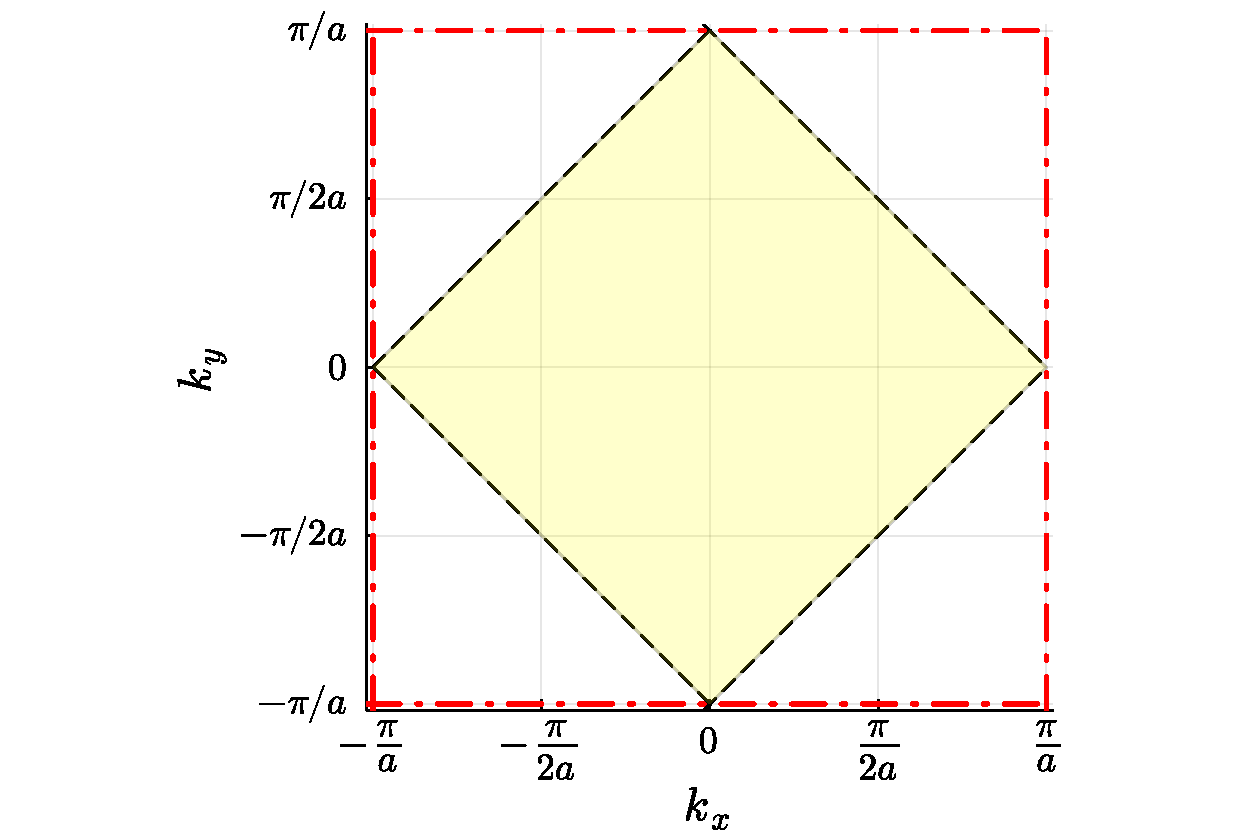
\includegraphics[scale=0.5]{Q2(fermi).pdf}
    \caption{\textbf{Fermi surface for square lattice}. The red lines denote the BZ while the Fermi-surface is denoted by the black dashed lines. The yellow shaded region denotes the filled Fermi sea.}
\end{figure}

\noindent
\underline{\textbf{{\sffamily Solution 3: Tight Binding with Modulated On-site Potential}}}
\\[0.2cm]
% % \begin{definition}[]
% %     Consider the one-dimensional tight-binding Hamiltonian that includes an additional modulated on-site potential term,
% % \[
% % \hat{H}=-t\sum_{n}(|n\rangle\langle n+1|+\text{h.c.})+U\sum_{n}|n \rangle\langle n|+V\sum_{n}(-1)^{n}|n\rangle\langle n|.
% % \]

% % \begin{enumerate}
% %     \item[(a)] Determine the dispersion relation corresponding to this Hamiltonian.
    
% %     \item[(b)] Further, demonstrate that the Brillouin zone becomes reduced as a result of the staggered potential. 
% % \end{enumerate}
% % \end{definition}
% \noindent
% \textit{Answer.}
\noindent
The given Hamiltonian can be schematically represented as below, where between each site, the hopping amplitude is $-t$ and the onsite-potential is $U$ and an additional on-site potential of strength $V$ is imposed with alternate signs along the sites. 
\begin{figure}[H]
    \centering
    

\tikzset{every picture/.style={line width=0.75pt}} %set default line width to 0.75pt        

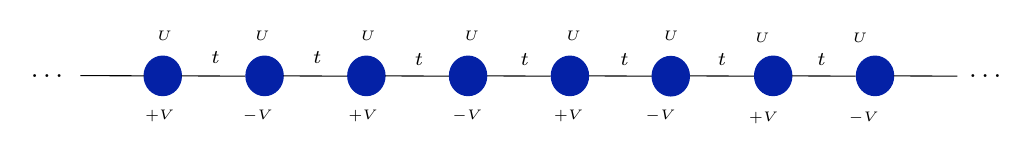
\begin{tikzpicture}[x=0.75pt,y=0.75pt,yscale=-1,xscale=1]
%uncomment if require: \path (0,179); %set diagram left start at 0, and has height of 179

%Shape: Ellipse [id:dp36206324476607865] 
\draw  [color={rgb, 255:red, 4; green, 33; blue, 166 }  ,draw opacity=1 ][fill={rgb, 255:red, 4; green, 33; blue, 166 }  ,fill opacity=1 ] (113.81,106.35) .. controls (113.81,101.09) and (117.84,96.82) .. (122.81,96.82) .. controls (127.78,96.82) and (131.81,101.09) .. (131.81,106.35) .. controls (131.81,111.62) and (127.78,115.88) .. (122.81,115.88) .. controls (117.84,115.88) and (113.81,111.62) .. (113.81,106.35) -- cycle ;
%Straight Lines [id:da04431193308496273] 
\draw    (131.81,106.35) -- (162.51,106.5) ;
%Shape: Ellipse [id:dp3003453169599384] 
\draw  [color={rgb, 255:red, 4; green, 33; blue, 166 }  ,draw opacity=1 ][fill={rgb, 255:red, 4; green, 33; blue, 166 }  ,fill opacity=1 ] (162.87,106.35) .. controls (162.87,101.09) and (166.89,96.82) .. (171.87,96.82) .. controls (176.84,96.82) and (180.87,101.09) .. (180.87,106.35) .. controls (180.87,111.62) and (176.84,115.88) .. (171.87,115.88) .. controls (166.89,115.88) and (162.87,111.62) .. (162.87,106.35) -- cycle ;
%Straight Lines [id:da7024556631331752] 
\draw    (180.87,106.35) -- (211.57,106.5) ;
%Shape: Ellipse [id:dp2794537122205859] 
\draw  [color={rgb, 255:red, 4; green, 33; blue, 166 }  ,draw opacity=1 ][fill={rgb, 255:red, 4; green, 33; blue, 166 }  ,fill opacity=1 ] (211.92,106.35) .. controls (211.92,101.09) and (215.95,96.82) .. (220.92,96.82) .. controls (225.89,96.82) and (229.92,101.09) .. (229.92,106.35) .. controls (229.92,111.62) and (225.89,115.88) .. (220.92,115.88) .. controls (215.95,115.88) and (211.92,111.62) .. (211.92,106.35) -- cycle ;
%Straight Lines [id:da39368536495073636] 
\draw    (229.92,106.35) -- (260.63,106.5) ;
%Straight Lines [id:da595444549927224] 
\draw    (278.98,106.35) -- (309.68,106.5) ;
%Straight Lines [id:da2819209729867129] 
\draw    (83.1,106.2) -- (113.81,106.35) ;
%Straight Lines [id:da07405693969756366] 
\draw    (327.81,106.35) -- (358.51,106.5) ;
%Straight Lines [id:da588793866555433] 
\draw    (376.87,106.35) -- (407.57,106.5) ;
%Shape: Ellipse [id:dp4182973165942272] 
\draw  [color={rgb, 255:red, 4; green, 33; blue, 166 }  ,draw opacity=1 ][fill={rgb, 255:red, 4; green, 33; blue, 166 }  ,fill opacity=1 ] (407.92,106.35) .. controls (407.92,101.09) and (411.95,96.82) .. (416.92,96.82) .. controls (421.89,96.82) and (425.92,101.09) .. (425.92,106.35) .. controls (425.92,111.62) and (421.89,115.88) .. (416.92,115.88) .. controls (411.95,115.88) and (407.92,111.62) .. (407.92,106.35) -- cycle ;
%Straight Lines [id:da01335366634594748] 
\draw    (425.92,106.35) -- (456.63,106.5) ;
%Shape: Ellipse [id:dp3052794483264457] 
\draw  [color={rgb, 255:red, 4; green, 33; blue, 166 }  ,draw opacity=1 ][fill={rgb, 255:red, 4; green, 33; blue, 166 }  ,fill opacity=1 ] (456.98,106.35) .. controls (456.98,101.09) and (461.01,96.82) .. (465.98,96.82) .. controls (470.95,96.82) and (474.98,101.09) .. (474.98,106.35) .. controls (474.98,111.62) and (470.95,115.88) .. (465.98,115.88) .. controls (461.01,115.88) and (456.98,111.62) .. (456.98,106.35) -- cycle ;
%Straight Lines [id:da0010409614992828997] 
\draw    (474.98,106.35) -- (505.68,106.5) ;
%Shape: Ellipse [id:dp6714313098237837] 
\draw  [color={rgb, 255:red, 4; green, 33; blue, 166 }  ,draw opacity=1 ][fill={rgb, 255:red, 4; green, 33; blue, 166 }  ,fill opacity=1 ] (260.92,106.35) .. controls (260.92,101.09) and (264.95,96.82) .. (269.92,96.82) .. controls (274.89,96.82) and (278.92,101.09) .. (278.92,106.35) .. controls (278.92,111.62) and (274.89,115.88) .. (269.92,115.88) .. controls (264.95,115.88) and (260.92,111.62) .. (260.92,106.35) -- cycle ;
%Shape: Ellipse [id:dp854641907197436] 
\draw  [color={rgb, 255:red, 4; green, 33; blue, 166 }  ,draw opacity=1 ][fill={rgb, 255:red, 4; green, 33; blue, 166 }  ,fill opacity=1 ] (309.98,106.35) .. controls (309.98,101.09) and (314.01,96.82) .. (318.98,96.82) .. controls (323.95,96.82) and (327.98,101.09) .. (327.98,106.35) .. controls (327.98,111.62) and (323.95,115.88) .. (318.98,115.88) .. controls (314.01,115.88) and (309.98,111.62) .. (309.98,106.35) -- cycle ;
%Shape: Ellipse [id:dp43489024391922837] 
\draw  [color={rgb, 255:red, 4; green, 33; blue, 166 }  ,draw opacity=1 ][fill={rgb, 255:red, 4; green, 33; blue, 166 }  ,fill opacity=1 ] (358.57,106.5) .. controls (358.57,101.24) and (362.6,96.97) .. (367.57,96.97) .. controls (372.54,96.97) and (376.57,101.24) .. (376.57,106.5) .. controls (376.57,111.77) and (372.54,116.04) .. (367.57,116.04) .. controls (362.6,116.04) and (358.57,111.77) .. (358.57,106.5) -- cycle ;

% Text Node
\draw (119,83.4) node [anchor=north west][inner sep=0.75pt]  [font=\tiny]  {$U$};
% Text Node
\draw (166,83.4) node [anchor=north west][inner sep=0.75pt]  [font=\tiny]  {$U$};
% Text Node
\draw (217,83.4) node [anchor=north west][inner sep=0.75pt]  [font=\tiny]  {$U$};
% Text Node
\draw (267,83.4) node [anchor=north west][inner sep=0.75pt]  [font=\tiny]  {$U$};
% Text Node
\draw (316,83.4) node [anchor=north west][inner sep=0.75pt]  [font=\tiny]  {$U$};
% Text Node
\draw (363,83.4) node [anchor=north west][inner sep=0.75pt]  [font=\tiny]  {$U$};
% Text Node
\draw (407,84.4) node [anchor=north west][inner sep=0.75pt]  [font=\tiny]  {$U$};
% Text Node
\draw (454,84.4) node [anchor=north west][inner sep=0.75pt]  [font=\tiny]  {$U$};
% Text Node
\draw (113,121.4) node [anchor=north west][inner sep=0.75pt]  [font=\tiny]  {$+V$};
% Text Node
\draw (160,121.4) node [anchor=north west][inner sep=0.75pt]  [font=\tiny]  {$-V$};
% Text Node
\draw (211,121.4) node [anchor=north west][inner sep=0.75pt]  [font=\tiny]  {$+V$};
% Text Node
\draw (261,121.4) node [anchor=north west][inner sep=0.75pt]  [font=\tiny]  {$-V$};
% Text Node
\draw (310,121.4) node [anchor=north west][inner sep=0.75pt]  [font=\tiny]  {$+V$};
% Text Node
\draw (354.19,121.4) node [anchor=north west][inner sep=0.75pt]  [font=\tiny,xslant=0.04]  {$-V$};
% Text Node
\draw (404,122.4) node [anchor=north west][inner sep=0.75pt]  [font=\tiny]  {$+V$};
% Text Node
\draw (452,122.4) node [anchor=north west][inner sep=0.75pt]  [font=\tiny]  {$-V$};
% Text Node
\draw (145,93.4) node [anchor=north west][inner sep=0.75pt]  [font=\scriptsize]  {$t$};
% Text Node
\draw (194,93.4) node [anchor=north west][inner sep=0.75pt]  [font=\scriptsize]  {$t$};
% Text Node
\draw (243,94.4) node [anchor=north west][inner sep=0.75pt]  [font=\scriptsize]  {$t$};
% Text Node
\draw (294,94.4) node [anchor=north west][inner sep=0.75pt]  [font=\scriptsize]  {$t$};
% Text Node
\draw (342,94.4) node [anchor=north west][inner sep=0.75pt]  [font=\scriptsize]  {$t$};
% Text Node
\draw (389,94.4) node [anchor=north west][inner sep=0.75pt]  [font=\scriptsize]  {$t$};
% Text Node
\draw (437,94.4) node [anchor=north west][inner sep=0.75pt]  [font=\scriptsize]  {$t$};
% Text Node
\draw (58,104.4) node [anchor=north west][inner sep=0.75pt]    {$\dotsc $};
% Text Node
\draw (510,104.4) node [anchor=north west][inner sep=0.75pt]    {$\dotsc $};


\end{tikzpicture}

\end{figure}
\noindent
We can equivalently divide the entire lattice into sublattices, where each unit cell now contains two atoms $A$ and $B$, as shown below: 
\begin{figure}[H]
    \centering
    \input{pics/q3_2.tex}
\end{figure}\noindent
where the red sites in the $j^{\text{\small th}}$ unit cell denote sublattice atoms of type $A$ (located at sites $2j$) and the blue sites denote sublattice atoms of type $B$ (located at sites $2j+1$). We can then define the lattice creation and annihilation operators for each sublattice sites viz. $\hat{c}\tund{A,i}^\dagger$ and $\hat{c}\tund{A,i}$ which will create and destroy particle at $A$ site of unit cell $i$ respectively and $\hat{c}\tund{B,i}^\dagger$ and $\hat{c}\tund{B,i}$ which will create and destroy particle at $B$ site of unit cell $i$. \\[0.2cm]
Dividing the lattice into two sublattices, we note that $+V$ ($-V$) now occurs only at site $A$ (site $B$) and then we can easily rewrite the above Hamiltonian as,
\begin{align*}
    \hat{H} = -t\sum\limits_{i}\qty(\craip \annbi + \text{h.c})  -t\sum\limits_{i}\qty(\crai \annbi + \text{h.c})  + (U+V)\sum\limits_{i}\crai \annai+(U-V)\sum\limits_{i}\crai \annai 
\end{align*} 
We can now expand these creation and annihilation operators in the momentum space as follows:
\begin{align*}
    \annar = \frac{1}{\sqrt{\sfrac{N}{2}}}\sum\limits_{k}e^{2ikra} \annak\qquad  \annbr = \frac{1}{\sqrt{\sfrac{N}{2}}}\sum\limits_{k}e^{2ikra} \annbk
\end{align*}
We now substitute this in the Hamiltonian above. Let us do this term-by-term, first for the hopping terms: 
\begin{align*}
    -t\sum\limits_{i}\qty(\craip \annbi +\crbi\annaip  ) &= -\frac{t}{\sqrt{\sfrac{N}{2}}}\sum\limits_{r,k,k'} e^{-2ika(r+1)} e^{2ik'ar} \crak \annbkd + e^{-2ik'ar}e^{2ika(r+1)} \crbkd \annak\\
    &= -\frac{t}{\sqrt{\sfrac{N}{2}}}\sum\limits_{r,k,k'} e^{-2ika}e^{-2ira(k-k')} \crak \annbkd + e^{2ika}e^{-2ira(k'-k)} \crbkd \annak\\
    &= -t\sum\limits_{k,k'} e^{-2ika}\delta_{k,k'} \crak \annbkd + e^{2ika}\delta_{k,k'}\crbkd \annak\\
    &=-t\sum\limits_{k} e^{-2ika} \crak \annbk + e^{2ika}\crbk \annak
\end{align*}
\begin{align*}
    -t\sum\limits_{i}\qty(\crai \annbi +\crbi\annai  ) &= -\frac{t}{\sqrt{\sfrac{N}{2}}}\sum\limits_{r,k,k'} e^{-2ikar} e^{2ik'ar} \crak \annbkd + e^{-2ik'ra}e^{2ikra} \crbkd \annak\\
    &= -\frac{t}{\sqrt{\sfrac{N}{2}}}\sum\limits_{r,k,k'} e^{-2ira(k-k')} \crak \annbkd + e^{-2ira(k'-k)} \crbkd \annak\\
    &= -t\sum\limits_{k,k'}  \crak \annbkd + \crbkd \annak\\
    &=-t\sum\limits_{k}  \crak \annbk + \crbk \annak
\end{align*}
Similarly the on-site terms would have a similar form:
\begin{align*}
    (U+V)\sum\limits_i \crai \annai  = (U+V)\sum\limits_{k} \crak \annak \qquad (U-V)\sum\limits_i \crai \annai  = (U-V)\sum\limits_{k} \crbk \annbk
\end{align*}
where we have used the identity that $\frac{1}{\sqrt{\sfrac{N}{2}}}\sum\limits_{r} e^{-2ia(k-k')r} = \delta_{k,k'}$. Now joining these terms together we get the following: 
\begin{align*}
    \hat{H} = \sum\limits_{k} -t(1+e^{-2ika}) \crak \annbk -t(1+e^{2ika})\crbk \annak (U+V)\crak \annak+(U-V)\crbk \annbk 
\end{align*}
Let us define the vector $\hat{\vb{c}}\tund{k}:= \mqty(\annak\\ \annbk)$ and then we can compactly write the Hamiltonian as: 
\begin{align*}
    \hat{H} = \sum\limits_{k} \hat{\vb{c}}\tund{k}^\dagger\ h(k) \ \hat{\vb{c}}\tund{k}
\end{align*}
where the matrix $h(k)$ takes the following form: 
$$h(k) = \mqty((U+V) & -t(1+e^{-2ika})\\ -t(1+e^{2ika})& (U-V))\quad \xrightarrow{\text{diagonalise}}\quad \det\mqty((U+V-\lambda) & -t(1+e^{-2ika})\\ -t(1+e^{2ika})& (U-V -\lambda)) =0$$
We obtain the characteristic equation as:
\begin{align*}
    (U-\lambda)^2 - V^2 -t^2(2+2\cos(2ka)) =0 \implies  (U-\lambda)^2 = V^2 +4t^2\cos^2(ka) 
\end{align*}
The dispersion relation obtained for the modulated on-site potential is  
$$\boxed{\lambda_{\pm}(k) = U\pm \sqrt{V^2 +4t^2\cos^2(ka)}}$$
Since we have two sublattices, we now get a two-band dispersion relation.
(b) If $V=0$ then the lattice has translational symmetry of unit $a$, however, when $V\neq 0$ then this translational symmetry becomes $2a$ (which we also saw explicitly from the sublattice structure). Thus the Brillouin zone reduces from $\qty(-\sfrac{\pi}{a},\sfrac{\pi}{a})$ to $\qty(-\sfrac{\pi}{2a},\sfrac{\pi}{2a})$ due to the introduction of the staggered potential.\\[0.2cm] 
% \begin{definition}[Ladder Lattice]
%     Consider a one-dimensional lattice composed of two parallel chains, where each chain corresponds to a distinct orbital -- the lower chain represents the \(p\)-orbital and the upper chain represents the \(s\)-orbital. Electrons can hop between neighbouring sites within the same chain, as well as between the two orbitals on the same site. Such a system can be described by the following tight-binding Hamiltonian:
% \[
% H = -t\sum_{n}\left(\left|n,s\right\rangle\left\langle n+1,s\right|+ \text{h.c.}\right)-t^{\prime}\sum_{n}\left(\left|n,p\right\rangle\left\langle n +1,p\right|+\text{h.c.}\right)
% \]
% \[
% -\Omega\sum_{n}\left(\left|n,s\right\rangle\left\langle n,p\right |+\text{h.c.}\right)+{\varepsilon}_{s}\sum_{n}\left|n,s\right\rangle\left\langle n ,s\right|+{\varepsilon}_{p}\sum_{n}\left|n,p\right\rangle\left\langle n,p\right|.
% \]
% Here, \(t\) and \(t^{\prime}\) denote the hopping amplitudes along the \(s\) and \(p\) orbital chains, respectively, \(\Omega\) represents the inter-orbital coupling between the two chains, and \({\varepsilon}_{s}\) and \({\varepsilon}_{p}\) are the on-site energies of the respective orbitals.

% \begin{enumerate}
%     \item[(a)] Perform a Fourier transform to momentum space using the Bloch states
%     \[
%     \left|k,\sigma\right\rangle=\frac{1}{\sqrt{N}}\sum_{n}e^{ikns}\left|n,\sigma\right\rangle,
%     \]
%     where \(\sigma=s,p\), and express the Hamiltonian as a \(2\times 2\) matrix \(H(k)\).
    
%     \item[(b)] Obtain the energy dispersion relation \(E_{\pm}(s)\) and sketch the two resulting energy bands for representative parameters (\(t^{\prime}<t\), \(\Omega\neq 0\)).
% \end{enumerate}
   
% \end{definition}
% \noindent
%     \textit{Answer.}
\noindent 
\noindent
\underline{\textbf{{\sffamily Solution 4: Ladder Lattice}}}
\\[0.3cm]
The lattice can be schematically shown as: 
     \begin{figure}[H]
        \centering
    

\tikzset{every picture/.style={line width=0.75pt}} %set default line width to 0.75pt        

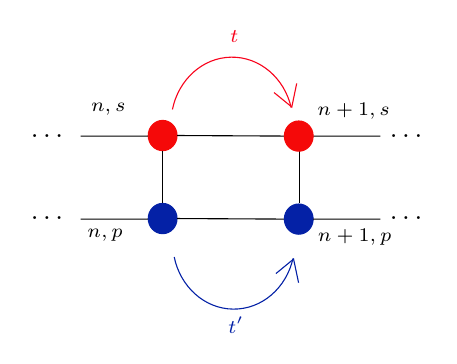
\begin{tikzpicture}[x=0.75pt,y=0.75pt,yscale=-1,xscale=1]
%uncomment if require: \path (0,221); %set diagram left start at 0, and has height of 221

%Shape: Ellipse [id:dp9509974546511886] 
\draw  [color={rgb, 255:red, 245; green, 9; blue, 9 }  ,draw opacity=1 ][fill={rgb, 255:red, 245; green, 9; blue, 9 }  ,fill opacity=1 ] (260.83,66.09) .. controls (260.83,62.08) and (263.93,58.82) .. (267.75,58.82) .. controls (271.58,58.82) and (274.68,62.08) .. (274.68,66.09) .. controls (274.68,70.11) and (271.58,73.37) .. (267.75,73.37) .. controls (263.93,73.37) and (260.83,70.11) .. (260.83,66.09) -- cycle ;
%Straight Lines [id:da6108239084572175] 
\draw    (274.68,66.09) -- (326.4,66.36) ;
%Shape: Ellipse [id:dp6505599276771276] 
\draw  [color={rgb, 255:red, 4; green, 33; blue, 166 }  ,draw opacity=1 ][fill={rgb, 255:red, 4; green, 33; blue, 166 }  ,fill opacity=1 ] (260.83,106.09) .. controls (260.83,102.08) and (263.93,98.82) .. (267.75,98.82) .. controls (271.58,98.82) and (274.68,102.08) .. (274.68,106.09) .. controls (274.68,110.11) and (271.58,113.37) .. (267.75,113.37) .. controls (263.93,113.37) and (260.83,110.11) .. (260.83,106.09) -- cycle ;
%Straight Lines [id:da5080637952717771] 
\draw    (274.68,106.09) -- (326.4,106.36) ;
%Shape: Ellipse [id:dp6408999392104522] 
\draw  [color={rgb, 255:red, 4; green, 33; blue, 166 }  ,draw opacity=1 ][fill={rgb, 255:red, 4; green, 33; blue, 166 }  ,fill opacity=1 ] (326.4,106.36) .. controls (326.4,102.34) and (329.51,99.09) .. (333.33,99.09) .. controls (337.16,99.09) and (340.26,102.34) .. (340.26,106.36) .. controls (340.26,110.38) and (337.16,113.64) .. (333.33,113.64) .. controls (329.51,113.64) and (326.4,110.38) .. (326.4,106.36) -- cycle ;
%Straight Lines [id:da9048962890563637] 
\draw    (340.26,66.36) -- (372.68,66.37) ;
%Straight Lines [id:da8974227202113937] 
\draw    (340.26,106.36) -- (372.68,106.37) ;
%Straight Lines [id:da6458660967437829] 
\draw    (228.26,66.36) -- (260.68,66.37) ;
%Straight Lines [id:da235583538860336] 
\draw    (228.26,106.36) -- (260.68,106.37) ;
%Straight Lines [id:da13127610214656893] 
\draw    (267.75,73.37) -- (267.75,98.82) ;
%Straight Lines [id:da41734146815277795] 
\draw    (333.75,73.37) -- (333.75,98.82) ;
%Shape: Ellipse [id:dp9917459854521972] 
\draw  [color={rgb, 255:red, 245; green, 9; blue, 9 }  ,draw opacity=1 ][fill={rgb, 255:red, 245; green, 9; blue, 9 }  ,fill opacity=1 ] (326.4,66.36) .. controls (326.4,62.34) and (329.51,59.09) .. (333.33,59.09) .. controls (337.16,59.09) and (340.26,62.34) .. (340.26,66.36) .. controls (340.26,70.38) and (337.16,73.64) .. (333.33,73.64) .. controls (329.51,73.64) and (326.4,70.38) .. (326.4,66.36) -- cycle ;
%Shape: Arc [id:dp9460179479043493] 
\draw  [draw opacity=0] (329.7,52.67) .. controls (326.46,38.51) and (314.67,28.12) .. (300.76,28.34) .. controls (286.87,28.56) and (275.36,39.3) .. (272.47,53.53) -- (301.18,60.54) -- cycle ; \draw  [color={rgb, 255:red, 248; green, 3; blue, 28 }  ,draw opacity=1 ] (329.7,52.67) .. controls (326.46,38.51) and (314.67,28.12) .. (300.76,28.34) .. controls (286.87,28.56) and (275.36,39.3) .. (272.47,53.53) ;  
\draw  [color={rgb, 255:red, 247; green, 7; blue, 29 }  ,draw opacity=1 ] (321.45,45.4) -- (329.98,52.36) -- (332.35,40.97) ;
%Shape: Arc [id:dp33186402587230834] 
\draw  [draw opacity=0] (330.57,125.31) .. controls (327.37,139.48) and (315.61,149.91) .. (301.7,149.73) .. controls (287.81,149.56) and (276.26,138.86) .. (273.33,124.63) -- (302.02,117.54) -- cycle ; \draw  [color={rgb, 255:red, 4; green, 33; blue, 166 }  ,draw opacity=1 ] (330.57,125.31) .. controls (327.37,139.48) and (315.61,149.91) .. (301.7,149.73) .. controls (287.81,149.56) and (276.26,138.86) .. (273.33,124.63) ;  
\draw  [color={rgb, 255:red, 4; green, 33; blue, 166 }  ,draw opacity=1 ] (322.33,132.61) -- (330.84,125.62) -- (333.25,137.01) ;

% Text Node
\draw (203,64.4) node [anchor=north west][inner sep=0.75pt]    {$\dotsc $};
% Text Node
\draw (203,103.8) node [anchor=north west][inner sep=0.75pt]    {$\dotsc $};
% Text Node
\draw (376,64.4) node [anchor=north west][inner sep=0.75pt]    {$\dotsc $};
% Text Node
\draw (247,81.4) node [anchor=north west][inner sep=0.75pt]  [font=\scriptsize]  {$\si{\ohm}$};
% Text Node
\draw (340,81.4) node [anchor=north west][inner sep=0.75pt]  [font=\scriptsize]  {$\si{\ohm}$};
% Text Node
\draw (299,14.4) node [anchor=north west][inner sep=0.75pt]  [font=\scriptsize,color={rgb, 255:red, 248; green, 3; blue, 28 }  ,opacity=1 ]  {$t$};
% Text Node
\draw (298,152.4) node [anchor=north west][inner sep=0.75pt]  [font=\scriptsize,color={rgb, 255:red, 4; green, 33; blue, 166 }  ,opacity=1 ]  {$t'$};
% Text Node
\draw (232,49.4) node [anchor=north west][inner sep=0.75pt]  [font=\scriptsize]  {$\ket{n,s}$};
% Text Node
\draw (230.26,109.76) node [anchor=north west][inner sep=0.75pt]  [font=\scriptsize]  {$\ket{n,p}$};
% Text Node
\draw (341.33,109.76) node [anchor=north west][inner sep=0.75pt]  [font=\scriptsize]  {$\ket{n+1,p}$};
% Text Node
\draw (341,49.4) node [anchor=north west][inner sep=0.75pt]  [font=\scriptsize]  {$\ket{n+1,s}$};
% Text Node
\draw (376,103.8) node [anchor=north west][inner sep=0.75pt]    {$\dotsc $};


\end{tikzpicture}

    \caption{Schematic representation of two coupled 1D chains corresponding to \(s\) and \(p\) orbitals. The hopping amplitudes along the \(s\) and \(p\) chains are \(t\) and \(t^{\prime}\) respectively, while the inter-chain coupling (hybridization) is \(\Omega\).
}
\end{figure} 
\noindent 
We can expand the orbital states in terms of the Fourier modes as, 
$$\ket{n,\sigma} = \frac{1}{\sqrt{N}}\sum\limits_{k} e^{-ikna}\ket{k,\sigma}$$
where $\sigma$ denotes the orbital type (\sigma \in \{s,p\}). Let us consider the terms of the Hamiltonian one by one.   
\begin{align*}
    -t \sum\limits_{n} \ket{n,s}\bra{n+1,s} + \ket{n+1,s}\bra{n,s} &= -\frac{t}{N}\sum\limits_{n,k,k'} (e^{-ikna} e^{ik'(n+1)a} + e^{-ik(n+1)a}e^{ik'na}) \ket{k,s}\bra{k',s}\\
    &=-\frac{t}{N}\sum\limits_{n,k,k'} (e^{ik'a} e^{-ina(k-k')} + e^{-ika}e^{-ina(k-k')}) \ket{k,s}\bra{k',s}\\
    &=-t \sum\limits_{k,k'} (e^{ik'a} \delta_{k,k'} + e^{-ika}\delta_{k,k'}) \ket{k,s}\bra{k',s}\\
     &=-t \sum\limits_{k} (e^{ika}  + e^{-ika}) \ket{k,s}\bra{k,s} = \sum\limits_{k}(-2t\cos(ka))\ket{k,s}\bra{k,s} 
\end{align*}
Similarly, the second term in the Hamiltonian leads to  
$$-t' \sum\limits_{n} \ket{n,p}\bra{n+1,p} + \ket{n+1,p}\bra{n,p} = \sum\limits_{k}(-2t'\cos(ka))\ket{k,p}\bra{k,p}$$
Let us now consider the onsite terms in the Hamiltonian:
\begin{align*}
    \varepsilon\tund{s}\sum\limits_n \ket{n,s}\bra{n,s} = \frac{ \varepsilon\tund{s}}{N}\sum\limits_{n,k,k'} e^{-ikna}e^{ik'na}\ket{k,s}\bra{k',s} = \frac{ \varepsilon\tund{s}}{N}\sum\limits_{n,k,k'} e^{-ina(k-k')}\ket{k,s}\bra{k',s} = \varepsilon\tund{s}\sum\limits_k \ket{k,s}\bra{k,s} 
\end{align*}
Similarly, for the $p$ orbital we will have the onsite term as: 
$$\varepsilon\tund{p}\sum\limits_n \ket{n,p}\bra{n,p} = \varepsilon\tund{p}\sum\limits_k \ket{k,p}\bra{k,p} $$
Finally, let us consider the hopping term between the parallel chains: 
\begin{align*}
    \Omega \sum\limits_n \ket{n,s}\bra{n,p} + \ket{n,p}\bra{n,s} &= -\frac{\Omega}{N} \sum\limits_{n,k,k'} e^{-ikna} e^{ik'na} \ket{k,s}\bra{k',p} + e^{-ikna} e^{ik'na} \ket{k,p}\bra{k',s} \\
    &= -\frac{\Omega}{N} \sum\limits_{n,k,k'} e^{-i(k-k')na} \qty[ \ket{k,s}\bra{k',p} +\ket{k,p}\bra{k',s}]\\
    &=-\Omega \sum\limits_k \ket{k,s}\bra{k,p} + \ket{k,p}\bra{k,s}
\end{align*}
Now joining all these terms together we get the Hamiltonian expanded in the momentum space as, 
\begin{align*}
    \hat{H} = \sum\limits_k (\varepsilon\tund{p}-2t'\cos(ka)) \ket{k,p}\bra{k,p} +(\varepsilon\tund{s}-2t\cos(ka)) \ket{k,s}\bra{k,s} -\Omega \ket{k,s}\bra{k,p} -\Omega \ket{k,p}\bra{k,s}
\end{align*}
Now using the fact that $\braket{q,\sigma|q',\sigma'} = \delta_{\sigma \sigma'}\delta_{q,q'}$ we can obtain the matrix elements: 
\begin{alignat*}{3}
     &\vartriangleright\ \braket{k',s|\hat{H}|k',s}  = \varepsilon\tund{s}-2t\cos(k'a)\qquad &&\vartriangleright\braket{k',s|\hat{H}|k',p}  = -\Omega\\
   &\vartriangleright\ \braket{k',p|\hat{H}|k',p}  = \varepsilon\tund{p}-2t'\cos(k'a) \qquad &&\vartriangleright\ \braket{k',p|\hat{H}|k',s}  =-\Omega
\end{alignat*}
$$H(k) = \mqty(\varepsilon\tund{s}-2t\cos(ka) & -\Omega \\ -\Omega & \varepsilon\tund{p}-2t'\cos(ka))$$
(b) The energy dispersion is found from the eigenvalues of the above matrix $H(k)$. We obtain the characteristic equation using 
$$\det \mqty(\varepsilon\tund{s}-2t\cos(ka)-\lambda & -\Omega \\ -\Omega & \varepsilon\tund{p}-2t'\cos(ka)-\lambda) = 0  $$
Let us denote $h\tund{1} = 2t\cos(ka)$ and $h\tund{2} = 2t'\cos(ka)$ for simplicity. Then we have the equation as,
\begin{align*}
     (\lambda - \varepsilon\tund{s} +h\tund{1})(\lambda - \varepsilon\tund{p} +h\tund{2}) -\Omega^2 = 0 \implies   \lambda^2 - \lambda ( (\varepsilon\tund{p}+\varepsilon\tund{s}) - (h\tund{1}+h\tund{2}) ) + (h\tund{1}-\varepsilon\tund{s})(h\tund{2}-\varepsilon\tund{p})-\Omega^2 = 0
\end{align*}
The solutions to this quadratic equation are given as: 
\begin{align*}
   \boxed{ E_\pm = \frac{1}{2}\qty{( (\varepsilon\tund{p}+\varepsilon\tund{s}) - (h\tund{1}+h\tund{2}) ) \pm \sqrt{( (\varepsilon\tund{p}+\varepsilon\tund{s}) - (h\tund{1}+h\tund{2}) )^2 - 4\qty[(h\tund{1}-\varepsilon\tund{s})(h\tund{2}-\varepsilon\tund{p})-\Omega^2]}}}
\end{align*}
\begin{figure}[H]
    \centering 
    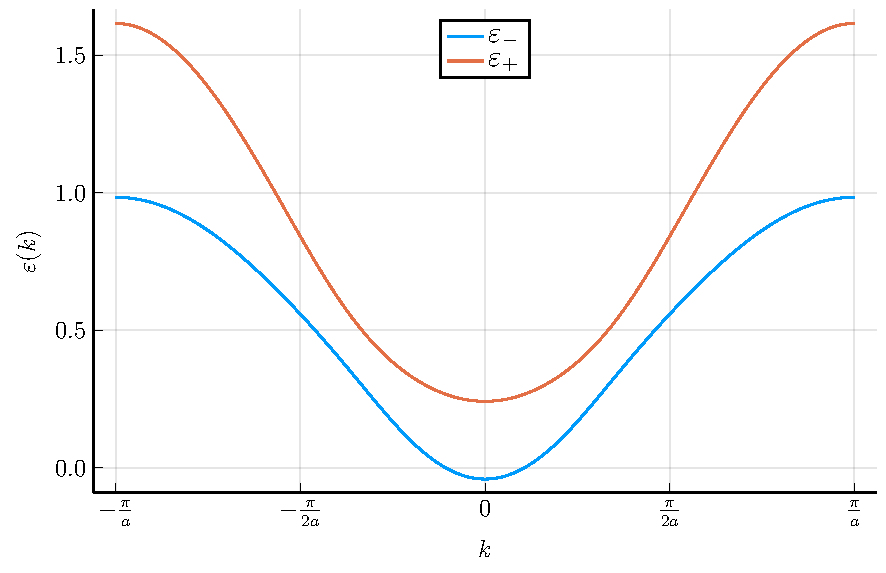
\includegraphics[scale=0.6]{Q4.pdf}
    \caption{\textbf{Dispersion for the ladder lattice.} The parameters used are $a=1,\varepsilon\tund{s} = 0.8, \varepsilon\tund{p}=0.6, t=0.4, t'=0.2, \Omega=0.1$}
\end{figure}


% \begin{definition}[Bloch's Theorem]
    
%     The wavefunction of a particle in a periodic lattice with lattice constant 'a' obeys Bloch's theorem,
% \[
% \psi_{n,k}(x)=e^{ikx}u_{n,k}(x),
% \]
% where \(u_{n,k}(x)\) has the periodicity of the lattice.

% \begin{enumerate}
%     \item[(a)] Substituting the Bloch form into the time-independent Schr\"{o}dinger equation, show that the problem reduces to
%     \[
%     h_{k}\,u_{n,k}(x)=\varepsilon\tund{n,k}\,u_{n,k}(x),\quad\text{where}\quad h_{k}=\frac {1}{2m}(p_{x}+\hbar k)^{2}+V(x),
%     \]
%     where the periodic potential can be expanded as
%     \[
%     V(x)=\sum_{G}V_{G}e^{iGx},
%     \]
%     where \(Ga=2\pi n\) are the reciprocal lattice vectors.
    
%     \item[(b)] Treating the potential \(V(x)\) as a weak perturbation, only the lowest harmonic is important
%     \[
%     V(x)\approx V_{G_{1}}e^{iG_{1}x}+V^{*}_{G_{1}}e^{-iG_{1}x}.
%     \]
%     (Since the potential is real, \(V^{*}_{G}=V_{-G}\)). Show that a gap of width \(\Delta=2|V_{G_{1}}|\) opens at the Brillouin zone boundary \(k=G_{1}/2\) (i.e., \(k=\pi/a\) for the first zone). Estimate \(\Delta\) from the truncated potential.
    
%     \item[(c)] For an optical lattice with a periodic Gaussian potential
%     \[
%     V(x)=-V_{0}\sum_{n}e^{-\alpha(x-na)^{2}},
%     \]
%     compute the Fourier coefficients \(V_{G}\) and hence estimate the band gap at the first zone boundary in the weak-potential limit.
    
%     \item[(d)] Extend the Bloch wave-vector into the complex plane as
%     \[
%     k=\frac{G}{2}+i\chi,\qquad\chi\in\mathcal{R},
%     \]
%     and repeat (b) to show that the allowed energies can exist within the forbidden region \(\Delta\), by suitably choosing \(\chi\).
% \end{enumerate}

% \end{definition}
% \noindent
% \textit{Answer}. 
\noindent
\underline{\textbf{{\sffamily Solution 5: Bloch's Theorem}}}
\\[0.3cm]
(a) Before substituting the equation in time-independent Schr{\"o}dinger, note that $$\hat{p}\equiv -i\hbar \partial_x \implies \hat{p}e^{ikx} = (-i\hbar) (ik) e^{ikx} = (\hbar k) e^{ikx}$$ Using this fact we can easily find that,
\begin{align*}
    \hat{p}^2 (e^{ikx} u_{n,k}(x)) &= \hat{p}\qty((\hbar k ) e^{ikx} u_{n,k} + e^{ikx}\hat{p}u_{n,k}) \\
    &=(\hbar k)\qty[(\hbar k)e^{ikx}u_{n,k} + e^{ikx} \hat{p}u_{n,k}] + (\hbar k)e^{ikx}\hat{p}u_{n,k} + e^{ikx} \hat{p}^2 u_{n,k}\\
    &=e^{ikx}[(\hbar k)^2 u_{n,k} + 2(\hbar k)\hat{p}u_{n,k} + \hat{p}^2 u_{n,k}] \equiv e^{ikx} (\hbar k + \hat{p})^2 u_{n,k}
\end{align*}
Hence we have 
\begin{align*}
    \hat{H} \psi_{n,k}(x) = \frac{\hat{p}^2}{2m}\psi_{n,k} + V(x)\psi_{n,k} =\cancel{e^{ikx}}\underbrace{\qty[ \frac{1}{2m}(\hbar k + \hat{p})^2+V(x)]}_{h_k} u_{n,k} = \varepsilon\tund{n,k} \cancel{e^{ikx}} u_{n,k} \implies \boxed{h_k u\tund{n,k}(x) = \varepsilon\tund{n,k}u\tund{n,k}(x)}
\end{align*}
(b) We now consider a perturbation with a weak potential such that only the lowest harmonic contributes to $V(x)$. We then have, 
\begin{align*}
    V(x) = V\tund{G\textsubscript{1}} e^{iG\textsubscript{\tiny 1} x}+V\tund{G\textsubscript{1}}^* e^{-iG\textsubscript{\tiny 1} x}
\end{align*}
where we have, for a general potential, $V(x) = \sum\limits_{\text{\tiny G}} V\tund{G}e^{i\text{\tiny G}x}$ and $G= \sfrac{2\pi n}{a}$ are the reciprocal lattice vectors. In the absence of the potential we have plane-wave solutions and the dispersion is quadratic, $\varepsilon(k)\sim k^2$ which implies that at the Brillouin zone boundaries $k = \pm \sfrac{\pi}{a} = \pm \sfrac{G\textsubscript{\tiny 1}}{2}$, we will have a degeneracy and thus we have to apply degenerate perturbation theory at the BZ boundaries! The unperturbed wavefunctions and energy at $ \pm \sfrac{G\textsubscript{\tiny 1}}{2} $ are: 
\begin{align*}
    \phi\tund{1}(x) =\frac{1}{\sqrt{L}} e^{i(G\tund{1}/2)x} \qquad  \phi\tund{2}(x) =\frac{1}{\sqrt{L}} e^{-i(G\tund{1}/2)x}\qquad; \quad \varepsilon\tund{0} = \frac{\hbar^2 G\tund{1}^2}{8m}
\end{align*}
where $L=Na$ is the length of the lattice. We have to diagonalise the potential in the degenerate subspace. For that consider $k = \sfrac{G\tund{1}}{2}$ and $k' =\sfrac{-G\tund{1}}{2} $
\begin{align*}
    \bra{k}H \ket{k} &= \frac{1}{L} \int\limits_{0}^L e^{-i(G\tund{1}/2)x} (\varepsilon\tund{0}+ V\tund{G\textsubscript{1}} e^{iG\textsubscript{\tiny 1} x}+V\tund{G\textsubscript{1}}^* e^{-iG\textsubscript{\tiny 1} x}) e^{i(G\tund{1}/2)x}\ \dd x \\
    &=\varepsilon\tund{0} + \frac{V\tund{G\textsubscript{1}}}{L} \qty[\frac{e^{iG\tund{1}x}}{iG\tund{1}}]_0^{L}+ \frac{V\tund{G\textsubscript{1}}^*}{L} \qty[\frac{e^{-iG\tund{1}x}}{-iG\tund{1}}]_0^{L}=\varepsilon\tund{0}
\end{align*}
since $G\tund{1} L = \frac{2\pi }{a}\times Na = 2\pi N \in \mathbb{N}$ and $\exp(2\pi n i)=1 \ \forall \ n\in \mathbb{Z}$. Similarly we have $\bra{k'}V \ket{k'} = \varepsilon\tund{0}$ by a similar calculation. Let us now consider the off-diagonal terms. 
\begin{align*}
    \bra{k'}H \ket{k} &= \frac{1}{L} \int\limits_{0}^L e^{i(G\tund{1}/2)x} (\varepsilon\tund{0}+ V\tund{G\textsubscript{1}} e^{iG\textsubscript{\tiny 1} x}+V\tund{G\textsubscript{1}}^* e^{-iG\textsubscript{\tiny 1} x}) e^{i(G\tund{1}/2)x}\ \dd x \\
    &= \frac{1}{L} \int\limits_{0}^L e^{iG\tund{1}x} (\varepsilon\tund{0}+ V\tund{G\textsubscript{1}} e^{iG\textsubscript{\tiny 1} x}+V\tund{G\textsubscript{1}}^* e^{-iG\textsubscript{\tiny 1} x}) \ \dd x = V\tund{G\textsubscript{1}}^*
\end{align*}
where the first two terms are zero (as shown before in the previous calculation) and the last term is only non-zero. We thus get $ \bra{k'}H \ket{k}  = V\tund{G\textsubscript{1}}^*$. Taking the Hermitian conjugate of this equation we have $ \bra{k}H \ket{k'}  = V\tund{G\textsubscript{1}}$. Then we get the effective matrix in the degenerate subspace as:
$$H\tund{sub} = \mqty(\varepsilon\tund{0} & V\tund{G\textsubscript{1}} \\ V\tund{G\textsubscript{1}}^* & \varepsilon\tund{0})$$
The eigenvalues of the matrix are found by solving:
$$(\lambda-\varepsilon\tund{0})^2 = |V\tund{G\textsubscript{1}}|^2\implies \lambda = \varepsilon\tund{0}\pm |V\tund{G\textsubscript{1}}|$$
Thus we see that a gap opens up at the zone boundary and $\Delta = 2|V\tund{G\textsubscript{1}}|$ is the gap between the energies obtained after the perturbation. 
\begin{figure}[H]
    \centering 


\tikzset{every picture/.style={line width=0.75pt}} %set default line width to 0.75pt        

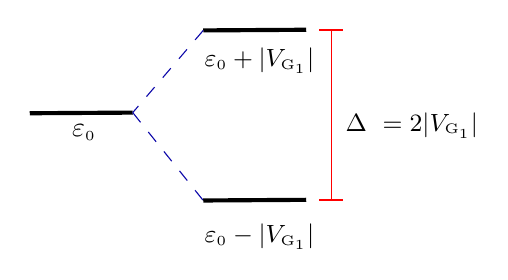
\begin{tikzpicture}[x=0.75pt,y=0.75pt,yscale=-1,xscale=1]
%uncomment if require: \path (0,324); %set diagram left start at 0, and has height of 324

%Straight Lines [id:da7088626522428005] 
\draw [line width=1.5]    (100,131.08) -- (149.62,130.77) ;
%Straight Lines [id:da4275212216468487] 
\draw [line width=1.5]    (183.59,91.17) -- (233.21,90.85) ;
%Straight Lines [id:da8539237829983396] 
\draw [line width=1.5]    (183.59,173.11) -- (233.21,172.79) ;
%Straight Lines [id:da21480704246896054] 
\draw [color={rgb, 255:red, 13; green, 8; blue, 169 }  ,draw opacity=1 ] [dash pattern={on 4.5pt off 4.5pt}]  (149.62,130.77) -- (183.59,173.11) ;
%Straight Lines [id:da164836390835303] 
\draw [color={rgb, 255:red, 13; green, 8; blue, 169 }  ,draw opacity=1 ] [dash pattern={on 4.5pt off 4.5pt}]  (183.59,91.17) -- (149.62,130.77) ;
%Straight Lines [id:da06528004783005803] 
\draw [color={rgb, 255:red, 255; green, 0; blue, 0 }  ,draw opacity=1 ]   (245.17,91.01) -- (245.17,172.95) ;
\draw [shift={(245.17,172.95)}, rotate = 270] [color={rgb, 255:red, 255; green, 0; blue, 0 }  ,draw opacity=1 ][line width=0.75]    (0,5.59) -- (0,-5.59)   ;
\draw [shift={(245.17,91.01)}, rotate = 270] [color={rgb, 255:red, 255; green, 0; blue, 0 }  ,draw opacity=1 ][line width=0.75]    (0,5.59) -- (0,-5.59)   ;

% Text Node
\draw (119.15,135.09) node [anchor=north west][inner sep=0.75pt]    {$\varepsilon\tund{0} $};
% Text Node
\draw (183,98.17) node [anchor=north west][inner sep=0.75pt]  [font=\small]  {$\varepsilon\tund{0} +|V\tund{G\textsubscript{1}}|$};
% Text Node
\draw (183,183.11) node [anchor=north west][inner sep=0.75pt]  [font=\small]  {$\varepsilon\tund{0} -|V\tund{G\textsubscript{1}}|$};
% Text Node
\draw (250.94,129.38) node [anchor=north west][inner sep=0.75pt]  [font=\small]  {$\Delta \ = 2|V\tund{G\textsubscript{1}}|$};


\end{tikzpicture}
\caption{Splitting of energy levels on introducing the perturbative weak-potential.}
\end{figure}
\noindent
(c) We have been given a periodic Gaussian potential 
$$V(x) = -V\tund{0}\sum\limits_n e^{-\alpha(x-na)^2}$$
We have to find the Fourier coefficients $V\tund{G}$ of this potential which are obtained as: 
$$V\tund{G}= \frac{1}{a}\int\limits_0^a \dd x \qty[-V\tund{0}\sum\limits_{n=-\infty}^{\infty}  e^{-\alpha(x-na)^2}] e^{-iGx} = -\frac{V\tund{0}}{a}\int\limits_0^a \dd x \qty[\sum\limits_{n=-\infty}^{\infty}  e^{-\alpha(x-na)^2}] e^{-iGx}$$
Let us substitute $y=x-na\longrightarrow \dd y = \dd x$. Then the coefficients becomes 
$$V\tund{G}=-\frac{V\tund{0}}{a}\sum\limits_{n=-\infty}^{\infty} \int\limits_{-na}^{a(1-n)} \dd y \ e^{-\alpha y^2} e^{-iG(y+na)}$$
Note that the integral is over a region of width $a$ and for different values of $n$, we obtain non-overlapping regions of width $a$. Thus, essentially, the sum and integral together forms the entire real line $\mathbb{R}$ and we can just replace the sum$+$integral with just an integral over the real line.\\[0.2cm]
Also note that the reciprocal lattice vectors are of the form $G=\sfrac{2\pi m}{a}$ and hence $Gna = 2\pi m n \implies e^{-iGna}=1$. Using these facts, we can write the coefficients as 

$$V\tund{G}=-\frac{V\tund{0}}{a}\int\limits_{-\infty}^{\infty} \dd y \ e^{-\alpha y^2} e^{-iGy}$$
The integral evaluates to $\sqrt{\frac{\pi}{\alpha}}e^{-G^2/4\alpha}$ and thus we get 
$$\boxed{V\tund{G}= -\frac{V\tund{0}}{a}\sqrt{\frac{\pi}{\alpha}}e^{-G^2/4\alpha}}$$
Then from the expression found out previously, for zone-boundary ($G=\sfrac{2\pi}{a}$) the band-gap becomes,
$$\boxed{\Delta = 2|V\tund{G\textsubscript{1}}| = \frac{2V\tund{0}}{a}\sqrt{\frac{\pi}{\alpha}}\ e^{-\pi^2/a^2\alpha}}$$
(d) Let us consider a complex wavevector of the form $k = \frac{G\tund{1}}{2}+i\chi$, which gives us 
$$\varepsilon\tund{0}(\pm k) = \frac{\hbar^2}{2m}\qty[\pm \frac{G\tund{1}}{2}+i\chi]^2 = \frac{\hbar^2}{2m} \qty[\qty(\frac{G\tund{1}}{2})^2 -\chi^2 \pm i\chi G\tund{1}]$$
The energies at the BZ boundaries now have a \textit{complex part}, however considering $\chi\ll G\tund{1}$ we can still use the perturbation theory. The Hamiltonian in the denegerate subspace now changes as: 
$$H\tund{sub} = \mqty(\varepsilon^{+}\tund{0} & V\tund{G\textsubscript{1}} \\ V\tund{G\textsubscript{1}}^* & \varepsilon\tund{0}^{-})$$
The eigenvalues are now found out from the characteristic equation, 
\begin{align*}
    \implies\quad &(\lambda -\varepsilon^{+}\tund{0})(\lambda -\varepsilon^{-}\tund{0}) - |V\tund{G\textsubscript{1}}|^2 =0\\
    \implies \quad & \lambda^2 - \lambda(\varepsilon^{+}\tund{0} + \varepsilon^{-}\tund{0}) +\varepsilon^{+}\tund{0}\varepsilon^{-}\tund{0} - |V\tund{G\textsubscript{1}}|^2=0\\
    \implies \quad & \lambda_{\pm} = \frac{1}{2}\qty{(\varepsilon^{+}\tund{0} + \varepsilon^{-}\tund{0}) \pm \sqrt{(\varepsilon^{+}\tund{0} + \varepsilon^{-}\tund{0})^2 - 4(\varepsilon^{+}\tund{0}\varepsilon^{-}\tund{0} - |V\tund{G\textsubscript{1}}|^2)}}\\
    &\hspace{0.2cm} = \frac{1}{2}\qty{(\varepsilon^{+}\tund{0} + \varepsilon^{-}\tund{0}) \pm \sqrt{(\varepsilon^{+}\tund{0} - \varepsilon^{-}\tund{0})^2 +4|V\tund{G\textsubscript{1}}|^2}}\\
    &\hspace{0.2cm} = \frac{\hbar^2}{2m}\qty[\qty(\frac{G\tund{1}}{2})^2 - \chi^2] \pm \sqrt{|V\tund{G\textsubscript{1}}|^2 - \qty(\frac{\hbar^2}{2m}\chi G\tund{1})^2}
\end{align*}
% Note that we can expand the second term in `small' $\chi$ limit,
% $$\sqrt{|V\tund{G\textsubscript{1}}|^2 - (\chi G\tund{1})^2} = |V\tund{G\textsubscript{1}}|\qty(1 - \frac{1}{2}\qty(\frac{\chi G\tund{1}}{|V\tund{G\textsubscript{1}}|})^2) = |V\tund{G\textsubscript{1}}| - \frac{1}{2}\frac{(\chi G\tund{1})^2}{|V\tund{G\textsubscript{1}}|}$$
By physical grounds, $\lambda\in \mathbb{R}$ and thus we have the following $$|V\tund{G\textsubscript{1}}|^2 \geq \qty(\frac{\hbar^2}{2m}\chi G\tund{1})^2\implies \chi \leq \frac{2m|V\tund{G\textsubscript{1}}|}{\hbar^2 G\tund{1}}\quad \text{or.}\quad \chi \geq -\frac{2 m|V\tund{G\textsubscript{1}}|}{\hbar^2 G\tund{1}}$$
Suppose we choose $\chi = \frac{2m|V\tund{G\textsubscript{1}}|}{\hbar^2 G\tund{1}}$ from which we get  $\lambda_{\pm} = \frac{h^2}{2m}\qty(\frac{G\tund{1}}{2})^2 -\frac{2m}{\hbar^2} \qty(\frac{ |V\tund{G\textsubscript{1}}|}{ G\tund{1}})^2$, which for `small' enough $\sfrac{|V\tund{G\textsubscript{1}}|}{G\tund{1}}$, is equal to the energy without splitting in part (b). For any $\chi$, note that the square root term is always less than $|V\tund{G\textsubscript{1}}|$ and hence the splitting will be lesser than what was in part (b) and this state will be in the \textit{forbidden region}. Thus for any $k\in \mathbb{C}$ defined with appropriate chosen value of $\xi$, there is a continuous set of allowed energies inside the gap, parameterized by $\chi$.\\[0.2cm]
% \begin{definition}[Reciprocal Lattice]
% Consider a body-centered cubic (bcc) lattice with lattice constant $a$. Identify the primitive lattice vectors, determine the corresponding reciprocal lattice vectors, and identify the type of reciprocal lattice obtained. Repeat the calculation for a two-dimensional equilateral triangular lattice with lattice constant $a$.
% \end{definition}
% \textit{Answer.}\\[0.2cm]
\noindent
\underline{\textbf{{\sffamily Solution 6: Reciprocal Lattice}}}
\\[0.4cm]
$\blacktriangleright$ \textbf{Body-centered cubic}\\[0.2cm]
Let us consider the primitive unit cell for bcc lattice, such that each side of the cube is $a$ and let us consider the atom at the centre of the cube to be the origin.
\begin{figure}[H]
    \centering 
    

\tikzset{every picture/.style={line width=0.75pt}} %set default line width to 0.75pt        

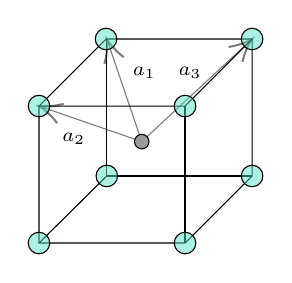
\begin{tikzpicture}[x=0.75pt,y=0.75pt,yscale=-1,xscale=1]
%uncomment if require: \path (0,188); %set diagram left start at 0, and has height of 188

%Straight Lines [id:da9706510828893629] 
\draw [color={rgb, 255:red, 0; green, 0; blue, 0 }  ,draw opacity=0.51 ]   (245.89,73.02) -- (293.51,89.49) ;
\draw [shift={(244,72.37)}, rotate = 19.08] [color={rgb, 255:red, 0; green, 0; blue, 0 }  ,draw opacity=0.51 ][line width=0.75]    (10.93,-4.9) .. controls (6.95,-2.3) and (3.31,-0.67) .. (0,0) .. controls (3.31,0.67) and (6.95,2.3) .. (10.93,4.9)   ;
%Straight Lines [id:da7406975639367493] 
\draw [color={rgb, 255:red, 0; green, 0; blue, 0 }  ,draw opacity=0.51 ]   (345.22,41.42) -- (293.51,89.49) ;
\draw [shift={(346.68,40.06)}, rotate = 137.09] [color={rgb, 255:red, 0; green, 0; blue, 0 }  ,draw opacity=0.51 ][line width=0.75]    (10.93,-4.9) .. controls (6.95,-2.3) and (3.31,-0.67) .. (0,0) .. controls (3.31,0.67) and (6.95,2.3) .. (10.93,4.9)   ;
%Straight Lines [id:da5659810210148305] 
\draw [color={rgb, 255:red, 0; green, 0; blue, 0 }  ,draw opacity=0.51 ]   (277.33,41.95) -- (293.51,89.49) ;
\draw [shift={(276.68,40.06)}, rotate = 71.2] [color={rgb, 255:red, 0; green, 0; blue, 0 }  ,draw opacity=0.51 ][line width=0.75]    (10.93,-4.9) .. controls (6.95,-2.3) and (3.31,-0.67) .. (0,0) .. controls (3.31,0.67) and (6.95,2.3) .. (10.93,4.9)   ;
%Shape: Cube [id:dp1265188075253546] 
\draw   (244,72.37) -- (276.31,40.06) -- (346.68,40.06) -- (346.68,106.06) -- (314.37,138.37) -- (244,138.37) -- cycle ; \draw   (346.68,40.06) -- (314.37,72.37) -- (244,72.37) ; \draw   (314.37,72.37) -- (314.37,138.37) ;
%Shape: Right Angle [id:dp7070065882483361] 
\draw   (346.68,106.06) -- (276.68,106.06) -- (276.68,40.06) ;
%Straight Lines [id:da062218437431547646] 
\draw    (276.68,106.06) -- (244,138.37) ;
%Shape: Circle [id:dp11648101603290684] 
\draw  [color={rgb, 255:red, 0; green, 0; blue, 0 }  ,draw opacity=1 ][fill={rgb, 255:red, 155; green, 155; blue, 155 }  ,fill opacity=1 ] (290.02,89.49) .. controls (290.02,87.56) and (291.58,86) .. (293.51,86) .. controls (295.44,86) and (297,87.56) .. (297,89.49) .. controls (297,91.42) and (295.44,92.98) .. (293.51,92.98) .. controls (291.58,92.98) and (290.02,91.42) .. (290.02,89.49) -- cycle ;
%Shape: Circle [id:dp11896613069123829] 
\draw  [fill={rgb, 255:red, 80; green, 227; blue, 194 }  ,fill opacity=0.48 ] (309.19,72.37) .. controls (309.19,69.5) and (311.51,67.18) .. (314.37,67.18) .. controls (317.24,67.18) and (319.56,69.5) .. (319.56,72.37) .. controls (319.56,75.23) and (317.24,77.55) .. (314.37,77.55) .. controls (311.51,77.55) and (309.19,75.23) .. (309.19,72.37) -- cycle ;
%Shape: Circle [id:dp947899176730009] 
\draw  [fill={rgb, 255:red, 80; green, 227; blue, 194 }  ,fill opacity=0.48 ] (341.5,40.06) .. controls (341.5,37.19) and (343.82,34.87) .. (346.68,34.87) .. controls (349.55,34.87) and (351.87,37.19) .. (351.87,40.06) .. controls (351.87,42.92) and (349.55,45.24) .. (346.68,45.24) .. controls (343.82,45.24) and (341.5,42.92) .. (341.5,40.06) -- cycle ;
%Shape: Circle [id:dp2317325899712206] 
\draw  [fill={rgb, 255:red, 80; green, 227; blue, 194 }  ,fill opacity=0.48 ] (271.13,40.06) .. controls (271.13,37.19) and (273.45,34.87) .. (276.31,34.87) .. controls (279.17,34.87) and (281.49,37.19) .. (281.49,40.06) .. controls (281.49,42.92) and (279.17,45.24) .. (276.31,45.24) .. controls (273.45,45.24) and (271.13,42.92) .. (271.13,40.06) -- cycle ;
%Shape: Circle [id:dp7716974761663259] 
\draw  [fill={rgb, 255:red, 80; green, 227; blue, 194 }  ,fill opacity=0.48 ] (238.82,72.37) .. controls (238.82,69.5) and (241.14,67.18) .. (244,67.18) .. controls (246.86,67.18) and (249.18,69.5) .. (249.18,72.37) .. controls (249.18,75.23) and (246.86,77.55) .. (244,77.55) .. controls (241.14,77.55) and (238.82,75.23) .. (238.82,72.37) -- cycle ;
%Shape: Circle [id:dp5766540400182227] 
\draw  [fill={rgb, 255:red, 80; green, 227; blue, 194 }  ,fill opacity=0.48 ] (238.82,138.37) .. controls (238.82,135.5) and (241.14,133.18) .. (244,133.18) .. controls (246.86,133.18) and (249.18,135.5) .. (249.18,138.37) .. controls (249.18,141.23) and (246.86,143.55) .. (244,143.55) .. controls (241.14,143.55) and (238.82,141.23) .. (238.82,138.37) -- cycle ;
%Shape: Circle [id:dp9156391300762504] 
\draw  [fill={rgb, 255:red, 80; green, 227; blue, 194 }  ,fill opacity=0.48 ] (309.19,138.37) .. controls (309.19,135.5) and (311.51,133.18) .. (314.37,133.18) .. controls (317.24,133.18) and (319.56,135.5) .. (319.56,138.37) .. controls (319.56,141.23) and (317.24,143.55) .. (314.37,143.55) .. controls (311.51,143.55) and (309.19,141.23) .. (309.19,138.37) -- cycle ;
%Shape: Circle [id:dp20619261417646584] 
\draw  [fill={rgb, 255:red, 80; green, 227; blue, 194 }  ,fill opacity=0.48 ] (341.5,106.06) .. controls (341.5,103.19) and (343.82,100.87) .. (346.68,100.87) .. controls (349.55,100.87) and (351.87,103.19) .. (351.87,106.06) .. controls (351.87,108.92) and (349.55,111.24) .. (346.68,111.24) .. controls (343.82,111.24) and (341.5,108.92) .. (341.5,106.06) -- cycle ;
%Shape: Circle [id:dp5678888787226154] 
\draw  [fill={rgb, 255:red, 80; green, 227; blue, 194 }  ,fill opacity=0.48 ] (271.5,106.06) .. controls (271.5,103.19) and (273.82,100.87) .. (276.68,100.87) .. controls (279.55,100.87) and (281.87,103.19) .. (281.87,106.06) .. controls (281.87,108.92) and (279.55,111.24) .. (276.68,111.24) .. controls (273.82,111.24) and (271.5,108.92) .. (271.5,106.06) -- cycle ;

% Text Node
\draw (288,52.4) node [anchor=north west][inner sep=0.75pt]  [font=\scriptsize]  {$\vb{a}\tund{1}$};
\draw (310,52.4) node [anchor=north west][inner sep=0.75pt]  [font=\scriptsize]  {$\vb{a}\tund{3}$};
% Text Node
\draw (254,84.4) node [anchor=north west][inner sep=0.75pt]  [font=\scriptsize]  {$\vb{a}\tund{2}$};


\end{tikzpicture}

\end{figure}
\noindent
There are $8$ nearest neighbours of this atom and we choose three of them to be the \textit{primitive lattice vectors}. 
$$\vb{a}\tund{1} = \frac{a}{2}\mqty(-1\\ -1\\1)\qquad \vb{a}\tund{2} = \frac{a}{2}\mqty(1\\ -1\\1) \qquad \vb{a}\tund{3} = \frac{a}{2}\mqty(-1\\ 1\\1)$$ 
We calculate the volume $v = \vb{a}\tund{1}\cdot (\vb{a}\tund{2}\times\vb{a}\tund{3} ) = \sfrac{a^3}{2}$. From this we can calculate the \textit{reciprocal lattice vectors},
\begin{align*}
    \vb{b}\tund{1}&= \frac{2\pi (\vb{a}\tund{2}\times \vb{a}\tund{3})}{v} =\frac{2\pi}{a} \mqty(-1\\ -1 \\ 0)\\
     \vb{b}\tund{2}&= \frac{2\pi (\vb{a}\tund{3}\times \vb{a}\tund{1})}{v} =\frac{2\pi}{a}\mqty(1\\ 0 \\ 1)\\
      \vb{b}\tund{3}&= \frac{2\pi (\vb{a}\tund{1}\times \vb{a}\tund{2})}{v} =\frac{2\pi}{a}\mqty(0\\ 1 \\1)
\end{align*}
$\blacktriangleright$ \textbf{Triangular Lattice}\\[0.2cm]
Let us consider the primitive unit cell for the 2D triangular lattice, such that each side of the triangle is $a$.
\begin{figure}[H]
    \centering 
    

\tikzset{every picture/.style={line width=0.75pt}} %set default line width to 0.75pt        

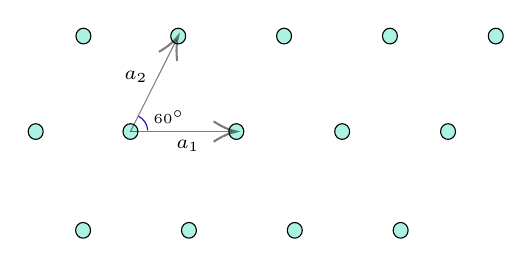
\begin{tikzpicture}[x=0.75pt,y=0.75pt,yscale=-1,xscale=1]
%uncomment if require: \path (0,300); %set diagram left start at 0, and has height of 300

%Shape: Ellipse [id:dp44540559931721835] 
\draw  [fill={rgb, 255:red, 80; green, 227; blue, 194 }  ,fill opacity=0.48 ] (184.82,48.6) .. controls (184.82,50.68) and (186.43,52.38) .. (188.42,52.38) .. controls (190.41,52.38) and (192.02,50.68) .. (192.02,48.6) .. controls (192.02,46.51) and (190.41,44.82) .. (188.42,44.82) .. controls (186.43,44.82) and (184.82,46.51) .. (184.82,48.6) -- cycle ;
%Shape: Ellipse [id:dp05735118303643005] 
\draw  [fill={rgb, 255:red, 80; green, 227; blue, 194 }  ,fill opacity=0.48 ] (230.48,48.6) .. controls (230.48,50.68) and (232.09,52.38) .. (234.08,52.38) .. controls (236.07,52.38) and (237.68,50.68) .. (237.68,48.6) .. controls (237.68,46.51) and (236.07,44.82) .. (234.08,44.82) .. controls (232.09,44.82) and (230.48,46.51) .. (230.48,48.6) -- cycle ;
%Shape: Ellipse [id:dp7910172309953121] 
\draw  [fill={rgb, 255:red, 80; green, 227; blue, 194 }  ,fill opacity=0.48 ] (281.48,48.6) .. controls (281.48,50.68) and (283.09,52.38) .. (285.08,52.38) .. controls (287.07,52.38) and (288.68,50.68) .. (288.68,48.6) .. controls (288.68,46.51) and (287.07,44.82) .. (285.08,44.82) .. controls (283.09,44.82) and (281.48,46.51) .. (281.48,48.6) -- cycle ;
%Shape: Ellipse [id:dp5268014214060158] 
\draw  [fill={rgb, 255:red, 80; green, 227; blue, 194 }  ,fill opacity=0.48 ] (332.48,48.6) .. controls (332.48,50.68) and (334.09,52.38) .. (336.08,52.38) .. controls (338.07,52.38) and (339.68,50.68) .. (339.68,48.6) .. controls (339.68,46.51) and (338.07,44.82) .. (336.08,44.82) .. controls (334.09,44.82) and (332.48,46.51) .. (332.48,48.6) -- cycle ;
%Shape: Ellipse [id:dp8337848758114892] 
\draw  [fill={rgb, 255:red, 80; green, 227; blue, 194 }  ,fill opacity=0.48 ] (383.48,48.6) .. controls (383.48,50.68) and (385.09,52.38) .. (387.08,52.38) .. controls (389.07,52.38) and (390.68,50.68) .. (390.68,48.6) .. controls (390.68,46.51) and (389.07,44.82) .. (387.08,44.82) .. controls (385.09,44.82) and (383.48,46.51) .. (383.48,48.6) -- cycle ;
%Shape: Ellipse [id:dp5233595101959089] 
\draw  [fill={rgb, 255:red, 80; green, 227; blue, 194 }  ,fill opacity=0.48 ] (184.65,142.19) .. controls (184.65,144.27) and (186.26,145.97) .. (188.25,145.97) .. controls (190.24,145.97) and (191.85,144.27) .. (191.85,142.19) .. controls (191.85,140.1) and (190.24,138.41) .. (188.25,138.41) .. controls (186.26,138.41) and (184.65,140.1) .. (184.65,142.19) -- cycle ;
%Shape: Ellipse [id:dp3261137816149532] 
\draw  [fill={rgb, 255:red, 80; green, 227; blue, 194 }  ,fill opacity=0.48 ] (161.82,94.6) .. controls (161.82,96.68) and (163.43,98.38) .. (165.42,98.38) .. controls (167.41,98.38) and (169.02,96.68) .. (169.02,94.6) .. controls (169.02,92.51) and (167.41,90.82) .. (165.42,90.82) .. controls (163.43,90.82) and (161.82,92.51) .. (161.82,94.6) -- cycle ;
%Shape: Ellipse [id:dp512976833325717] 
\draw  [fill={rgb, 255:red, 80; green, 227; blue, 194 }  ,fill opacity=0.48 ] (207.48,94.6) .. controls (207.48,96.68) and (209.09,98.38) .. (211.08,98.38) .. controls (213.07,98.38) and (214.68,96.68) .. (214.68,94.6) .. controls (214.68,92.51) and (213.07,90.82) .. (211.08,90.82) .. controls (209.09,90.82) and (207.48,92.51) .. (207.48,94.6) -- cycle ;
%Shape: Ellipse [id:dp49854981314808167] 
\draw  [fill={rgb, 255:red, 80; green, 227; blue, 194 }  ,fill opacity=0.48 ] (235.65,142.19) .. controls (235.65,144.27) and (237.26,145.97) .. (239.25,145.97) .. controls (241.24,145.97) and (242.85,144.27) .. (242.85,142.19) .. controls (242.85,140.1) and (241.24,138.41) .. (239.25,138.41) .. controls (237.26,138.41) and (235.65,140.1) .. (235.65,142.19) -- cycle ;
%Shape: Ellipse [id:dp3989542811514091] 
\draw  [fill={rgb, 255:red, 80; green, 227; blue, 194 }  ,fill opacity=0.48 ] (258.48,94.6) .. controls (258.48,96.68) and (260.09,98.38) .. (262.08,98.38) .. controls (264.07,98.38) and (265.68,96.68) .. (265.68,94.6) .. controls (265.68,92.51) and (264.07,90.82) .. (262.08,90.82) .. controls (260.09,90.82) and (258.48,92.51) .. (258.48,94.6) -- cycle ;
%Shape: Ellipse [id:dp8803221961184908] 
\draw  [fill={rgb, 255:red, 80; green, 227; blue, 194 }  ,fill opacity=0.48 ] (286.65,142.19) .. controls (286.65,144.27) and (288.26,145.97) .. (290.25,145.97) .. controls (292.24,145.97) and (293.85,144.27) .. (293.85,142.19) .. controls (293.85,140.1) and (292.24,138.41) .. (290.25,138.41) .. controls (288.26,138.41) and (286.65,140.1) .. (286.65,142.19) -- cycle ;
%Shape: Ellipse [id:dp6294769569587648] 
\draw  [fill={rgb, 255:red, 80; green, 227; blue, 194 }  ,fill opacity=0.48 ] (309.48,94.6) .. controls (309.48,96.68) and (311.09,98.38) .. (313.08,98.38) .. controls (315.07,98.38) and (316.68,96.68) .. (316.68,94.6) .. controls (316.68,92.51) and (315.07,90.82) .. (313.08,90.82) .. controls (311.09,90.82) and (309.48,92.51) .. (309.48,94.6) -- cycle ;
%Shape: Ellipse [id:dp17018088276443522] 
\draw  [fill={rgb, 255:red, 80; green, 227; blue, 194 }  ,fill opacity=0.48 ] (337.65,142.19) .. controls (337.65,144.27) and (339.26,145.97) .. (341.25,145.97) .. controls (343.24,145.97) and (344.85,144.27) .. (344.85,142.19) .. controls (344.85,140.1) and (343.24,138.41) .. (341.25,138.41) .. controls (339.26,138.41) and (337.65,140.1) .. (337.65,142.19) -- cycle ;
%Shape: Ellipse [id:dp34571183004384987] 
\draw  [fill={rgb, 255:red, 80; green, 227; blue, 194 }  ,fill opacity=0.48 ] (360.48,94.6) .. controls (360.48,96.68) and (362.09,98.38) .. (364.08,98.38) .. controls (366.07,98.38) and (367.68,96.68) .. (367.68,94.6) .. controls (367.68,92.51) and (366.07,90.82) .. (364.08,90.82) .. controls (362.09,90.82) and (360.48,92.51) .. (360.48,94.6) -- cycle ;
%Straight Lines [id:da05891079864566384] 
\draw [color={rgb, 255:red, 0; green, 0; blue, 0 }  ,draw opacity=0.51 ]   (233.19,50.39) -- (211.08,94.6) ;
\draw [shift={(234.08,48.6)}, rotate = 116.57] [color={rgb, 255:red, 0; green, 0; blue, 0 }  ,draw opacity=0.51 ][line width=0.75]    (10.93,-4.9) .. controls (6.95,-2.3) and (3.31,-0.67) .. (0,0) .. controls (3.31,0.67) and (6.95,2.3) .. (10.93,4.9)   ;
%Straight Lines [id:da43172563314081036] 
\draw [color={rgb, 255:red, 0; green, 0; blue, 0 }  ,draw opacity=0.51 ]   (260.08,94.6) -- (211.08,94.6) ;
\draw [shift={(262.08,94.6)}, rotate = 180] [color={rgb, 255:red, 0; green, 0; blue, 0 }  ,draw opacity=0.51 ][line width=0.75]    (10.93,-4.9) .. controls (6.95,-2.3) and (3.31,-0.67) .. (0,0) .. controls (3.31,0.67) and (6.95,2.3) .. (10.93,4.9)   ;
%Shape: Arc [id:dp1289548304435324] 
\draw  [draw opacity=0] (214.96,87.21) .. controls (217.46,88.52) and (219.21,91.07) .. (219.4,94.04) -- (211.08,94.6) -- cycle ; \draw  [color={rgb, 255:red, 27; green, 5; blue, 191 }  ,draw opacity=1 ] (214.96,87.21) .. controls (217.46,88.52) and (219.21,91.07) .. (219.4,94.04) ;  

% Text Node
\draw (221,83.4) node [anchor=north west][inner sep=0.75pt]  [font=\tiny]  {$60^{\circ}$};
% Text Node
\draw (232,97.4) node [anchor=north west][inner sep=0.75pt]  [font=\scriptsize]  {$\vb{a}\tund{1}$};
% Text Node
\draw (207,64.4) node [anchor=north west][inner sep=0.75pt]  [font=\scriptsize]  {$\vb{a}\tund{2}$};


\end{tikzpicture}

\end{figure}
\noindent
There are $6$ nearest neighbours of an atom and we choose two of them to be the \textit{primitive lattice vectors}. 
$$\vb{a}\tund{1} = a\mqty(1\\ 0)\qquad \vb{a}\tund{2} = \frac{a}{2}\mqty(1\\ \sqrt{3}) $$ 
From the orthogonality relation we can say that the reciprocal lattice vectors, $\vb{b}\tund{1}\perp \vb{a}\tund{2}$ and $\vb{b}\tund{2}\perp \vb{a}\tund{1}$. Then suppose $\vb{b}\tund{1} = c(\sqrt{3}, -1)^{\text{\tiny T}}$ and $\vb{b}\tund{2} = d(0,-1)^{\text{\tiny T}}$. Moreover, from the normalisation we have, 
\begin{align*}
    \vb{a}\tund{1} \cdot   \vb{b}\tund{1} &=2\pi \implies c = \frac{2\pi}{\sqrt{3}a}\\
    \vb{a}\tund{2} \cdot   \vb{b}\tund{2} &=2\pi \implies d = -\frac{4\pi}{\sqrt{3}a}
\end{align*}
Thus we get the \textit{reciprocal lattice vectors} as 
$$\vb{b}\tund{1} = \frac{2\pi}{\sqrt{3}a}\mqty(\sqrt{3}\\ -1)\qquad \vb{b}\tund{2} = \frac{4\pi}{\sqrt{3}a}\mqty(0\\1)$$
% \begin{definition}[Ultracold Atoms]
% Ultracold atoms confined in an optical lattice experience a periodic potential given by  
% \[
% V(x) = V_0 \cos^2 \left( \frac{\pi x}{a} \right),
% \]  
% where \( V_0 \) is the lattice depth and \( a \) is the lattice spacing.  

% \begin{enumerate}
%     \item[(a)] Construct the Bloch wave function \(\Psi(x)\) for a particle in this lattice within the tight-binding approximation.
    
%     \item[(b)] Estimate the nearest-neighbour tunnelling amplitude \( t \), which characterises the hopping of an atom between adjacent lattice sites.
% \end{enumerate}
% \end{definition}
\noindent
\underline{\textbf{{\sffamily Solution 7: Ultracold Atoms}}}
\\[0.4cm]
Note that the minima of the given potential occurs at $x_n = \qty(n+\frac{1}{2})a$ and we can expand the potential about this minima, where from the Taylor series around $x_n$, we get, 
$$V(x) = V(x_n) + \dv{V}{x}\Bigg|_{x_n}(x-x_n)+ \frac{1}{2}\dv[2]{V}{x}\Bigg|_{x_n} (x-x_n)^2+\ldots$$
The first term vanishes as the minimum value of the potential is zero. The second term vanishes since at minima, the slope is zero. The quadratic term is:
$$ \frac{1}{2}\dv[2]{V}{x}\Bigg|_{x_n}= \frac{V\tund{0}}{2}\dv{x}\qty(-\frac{2\pi}{a}\cos(\frac{\pi x}{a})\sin(\frac{\pi x}{a}))\Bigg|_{x_n} = -\frac{\pi V\tund{0}}{2a}\dv{x}\qty(\sin\qty(\frac{2\pi x}{a}))\Bigg|_{x_n} =-\frac{\pi^2 V\tund{0}}{a^2}\cos(\frac{2\pi x}{a})\Bigg|_{x_n}  = \frac{\pi^2 }{a^2}V\tund{0}$$
Then we have an effective harmonic oscillator potential around each minima:
$$V(x) =  \frac{\pi^2 }{a^2}V\tund{0} (x-x_n)^2$$
Let us map the parameters with the usual SHO parameters: 
$$\frac{1}{2}m\omega^2 =  \frac{\pi^2 }{a^2}V\tund{0} \implies  \omega = \frac{\pi}{a}\sqrt{\frac{2V\tund{0}}{m}}$$
To construct the localised wavefunctions to expand the Bloch state, we can choose the ground state of the harmonic oscillator, since this potential is effectively harmonic.  
$$\varphi_n(x) = \qty(\frac{m\omega}{\pi \hbar})^{1/4} e^{-m\omega(x-x_n)^2/2\hbar}\longrightarrow \boxed{\varphi_n(x) = \frac{1}{(\pi \sigma^2)^{1/4}} e^{-(x-x_n)^2/2\sigma^2}}$$
where $\sigma = \sqrt{\sfrac{\hbar}{m\omega}} $ is the characteristic length scale of the system.
We can construct the Bloch wavefunction $\Psi_k(x)$ using a linear combination of these localised \textit{Wannier} functions in the tight-binding approximation. 
$$\Psi_k(x) = \frac{1}{\sqrt{N}}\sum\limits_n e^{ikna}\varphi_n(x)\ \ ;\quad \varphi_n(x) = \frac{1}{(\pi \sigma^2)^{1/4}} \exp\qty(-\frac{(x-x_n)^2}{2\sigma^2})$$
(b) Let us now calculate the tunneling amplitude $t$ which represents the probability of hopping between sites. Within the tight-binding approximation we only need to consider the nearest neighbour hopping and we have 
\begin{align*}
    t \approx - \braket{\varphi_n|\hat{H}|\varphi_{n+1}} = -\int\limits_{-\infty}^\infty \varphi_{n}^*(x) \qty(-\frac{\hbar^2}{2m}\dv[2]{x}+V(x))\varphi_{n+1}(x)
\end{align*}
Now consider the Hamiltonian for a harmonic oscillator centred at $x_{n+1}$ which can be written as:
$$\hat{H}_{n+1} = \hat{T}+ \frac{1}{2}m\omega^2 (x-x_{n+1})2 \implies \hat{H} = \hat{H}_{n+1}+(V - V_{n+1}) \equiv \hat{H}_{n+1}+\delta V_{n+1}$$
We can substitute this in the above integral and we obtain:
$$t\approx - \braket{\varphi_n|\hat{H}_{n+1}|\varphi_{n+1}} - \braket{\varphi_n|\delta V_{n+1}|\varphi_{n+1}} $$
Note that $\varphi_{n+1}$ is the ground state of $\hat{H}_{n+1}$ and thus the first term yields $-\varepsilon\tund{0} \braket{\varphi_n|\varphi_{n+1}}$ which is just the overlap between two Gaussian functions. Now let us come to the second term: 
 $$-\int\limits_{-\infty}^\infty \varphi_{n}^*(x) \ \delta V_{n+1}(x)\ \varphi_{n+1}(x)$$
 Note that, in the overlap region, that is, for $x$ between $x_{n}$ and $x_{n+1}$, the wavefunctions are negligible (since these are localised at the centres), although $\delta V$ is large (since there is significant deviation from the harmonic approximation), hence the integrand is negligible.\\[0.2cm] Moreover, around the centre $x_{n+1}$, the wavefunction $\varphi_{n+1}$ is large but $\delta V_{n+1}$ is small, since the harmonic approximation holds good around the centre. Around the centre $x_n$, $\delta V_{n+1}$ is large, but the wavefunction $\varphi_{n+1}$ is small. Hence in the region of importance, the integral is negligible and hence we can ignore this term from the tunneling amplitude.
 \begin{align*}
    \braket{\varphi_n|\varphi_{n+1}} = \frac{1}{\sqrt{\pi \sigma^2}}\int\limits_{-\infty}^{\infty} \exp\qty[-\frac{(x-x_n)^2}{2\sigma^2}]\exp\qty[-\frac{(x-x_{n+1})^2}{2\sigma^2}]
 \end{align*}
 Note the following: 
 \begin{align*}
    (x-A)^2+(x-B)^2 = 2(x^2 - x(A+B) +\frac{1}{2}(A^2+B^2)) &= 2\qty{\qty[x-\qty(\frac{A+B}{2})]^2 - \qty(\frac{A+B}{2})^2 + \frac{A^2+B^2}{2}}\\
   &= 2\qty{\qty[x-\qty(\frac{A+B}{2})]^2 -\frac{(A-B)^2}{4}}
 \end{align*}
 In our case we have $A=\qty(n+\frac{1}{2})a$ and $B=\qty(n+\frac{3}{2})a$ from which we get $A+B = 2(n+1)a$ and $B-A = a$. Then the overlap integral becomes:
 \begin{align*}
     \frac{1}{\sqrt{\pi \sigma^2}}\int\limits_{-\infty}^{\infty} \exp\qty[-\frac{1}{\sigma^2}\qty{\qty(x-(n+1)a)^2 - \frac{a^2}{4}}]= \frac{e^{-a^2/4\sigma^2}}{\sqrt{\pi \sigma^2}}\int\limits_{-\infty}^{\infty} \exp\qty[-\frac{1}{\sigma^2}\qty(x-(n+1)a)^2]
 \end{align*}
Let us make the substitution $y = \sqrt{2}(x-(n+1)a) \implies \dd y = \sqrt{2}\dd x$ and putting it in the integral we have the following expression, 
\begin{align*}
    \frac{e^{-a^2/4\sigma^2}}{\sqrt{2 \pi \sigma^2}}\int\limits_{-\infty}^{\infty} \exp\qty[-\frac{y^2}{2\sigma^2}] =\exp[-\frac{a^2}{4\sigma^2}]
\end{align*}
Then the tunneling amplitude is estimated as: 
$$\boxed{t\approx -\frac{\hbar\omega}{2}\exp[-\frac{a^2}{4\sigma^2}] = -\frac{\pi}{a}\sqrt{\frac{V\tund{0}\hbar^2}{2m}}\exp\qty[-\frac{\pi}{4}\sqrt{\frac{2V\tund{0}ma^2}{\hbar^2}}]}$$
Note that this amplitude is exponentially falling with $V\tund{0}$ which is nice, since for deep enough wells, the tight-binding approximation is expected to be valid. 
\end{document}